\documentclass[a4paper]{myarticle}

\title{CS7.302: Assignment 3}
\author{Himanshu Singh}
\date{February 17, 2024}

\begin{document}

\maketitle

\section{Pixel Subsampling for Anti-aliasing}

\subsection{Timings}

\begin{table}[H]
\centering
\renewcommand{\arraystretch}{1.5}
\begin{tabularx}{\linewidth}{LLL}
\hline
Scene & SPP & Render Time (ms) \\
\hline
\multirow{2}*{CornellBox: Directional Light} & 1 & 1037.84 \\
                          & 32 & 31507.78 \\
\hline
\end{tabularx}
\caption{Time taken for rendering models}
\end{table}

\subsection{Rendered Images}

\begin{figure}[H]
  \begin{minipage}[t]{.4\textwidth}
      \centering
      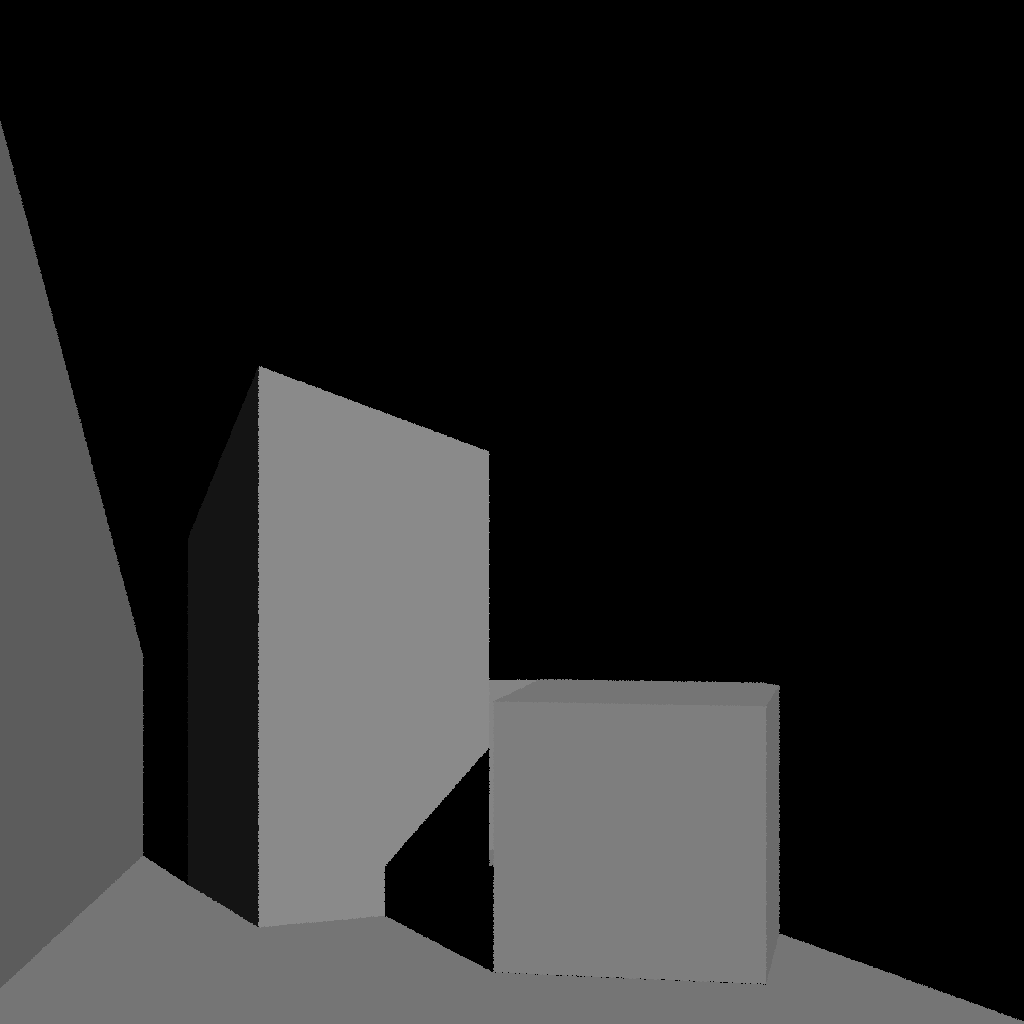
\includegraphics[width=\textwidth]{q1/cornell_box_1.png}
      \caption{Rendering of CornellBox, at 1 SPP}
  \end{minipage}
  \hfill
  \begin{minipage}[t]{.4\textwidth}
      \centering
      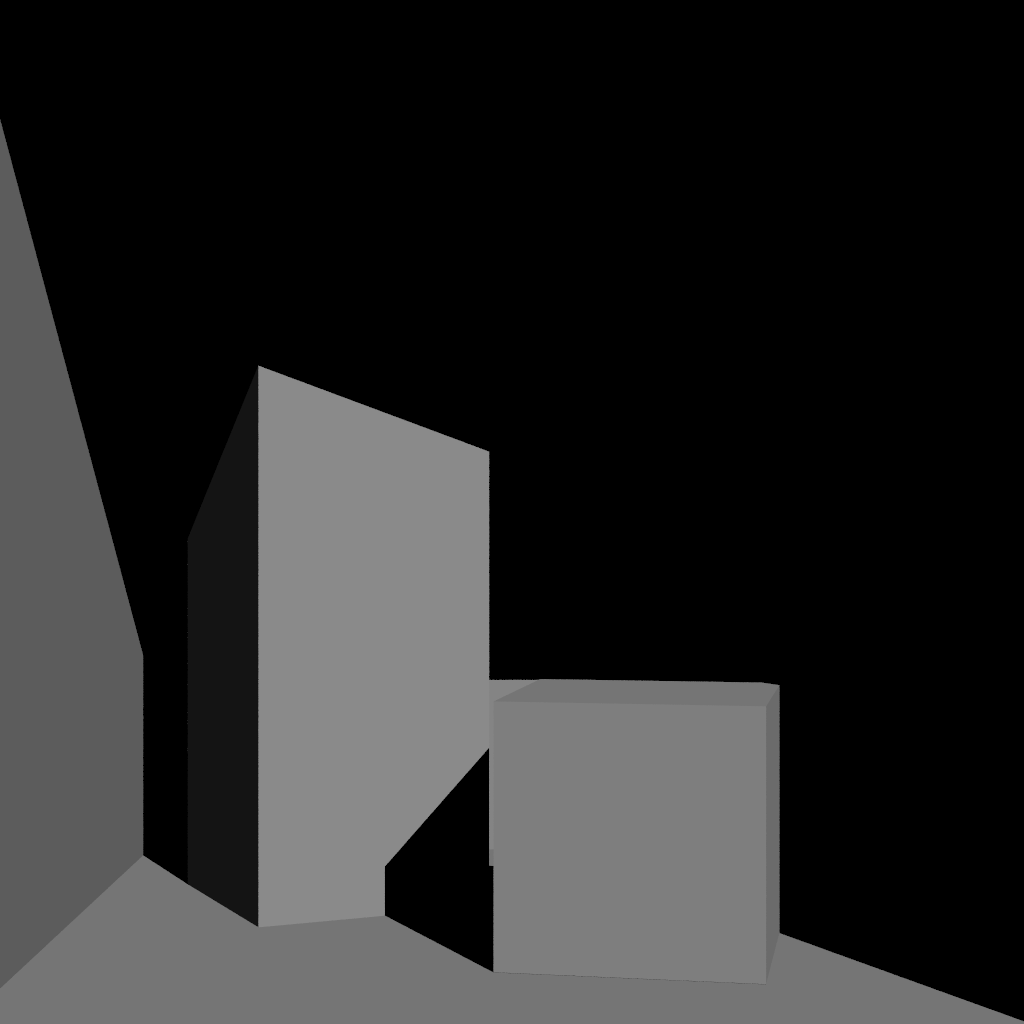
\includegraphics[width=\textwidth]{q1/cornell_box_32.png}
      \caption{Rendering of CornellBox, at 32 SPP}
  \end{minipage}
\end{figure}

\section{Area Light Support}

\subsection{Timings}

\begin{table}[H]
\centering
\renewcommand{\arraystretch}{1.5}
\begin{tabularx}{\linewidth}{LL}
\hline
Scene & Render Time (ms) \\
\hline
Scene 1 & 2966.52 \\
Scene 2 & 2564.13 \\
Scene 3 & 2788.72 \\
Scene 4 & 3544.12 \\
\hline
\end{tabularx}
\caption{Time taken for rendering models, with Area Light Support, at 32 SPP}
\end{table}

\subsection{Rendered Images}

\begin{figure}[H]
  \begin{minipage}[t]{.4\textwidth}
      \centering
      
\includegraphics[width=\textwidth]{q2/scene1.png}
      \caption{Rendering of Scene 1}
  \end{minipage}
  \hfill
  \begin{minipage}[t]{.4\textwidth}
      \centering
      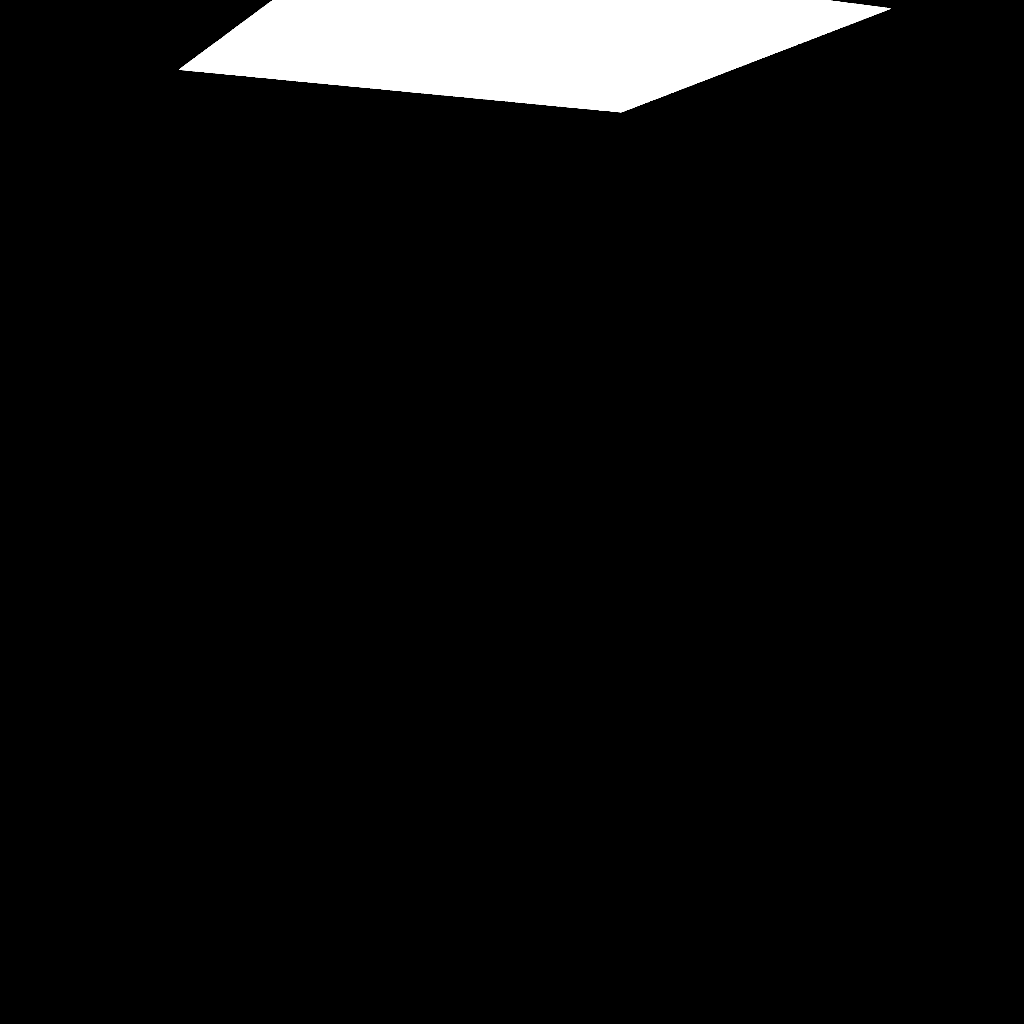
\includegraphics[width=\textwidth]{q2/scene2.png}
      \caption{Rendering of Scene 2}
  \end{minipage}
\end{figure}

\begin{figure}[H]
  \begin{minipage}[t]{.4\textwidth}
      \centering
      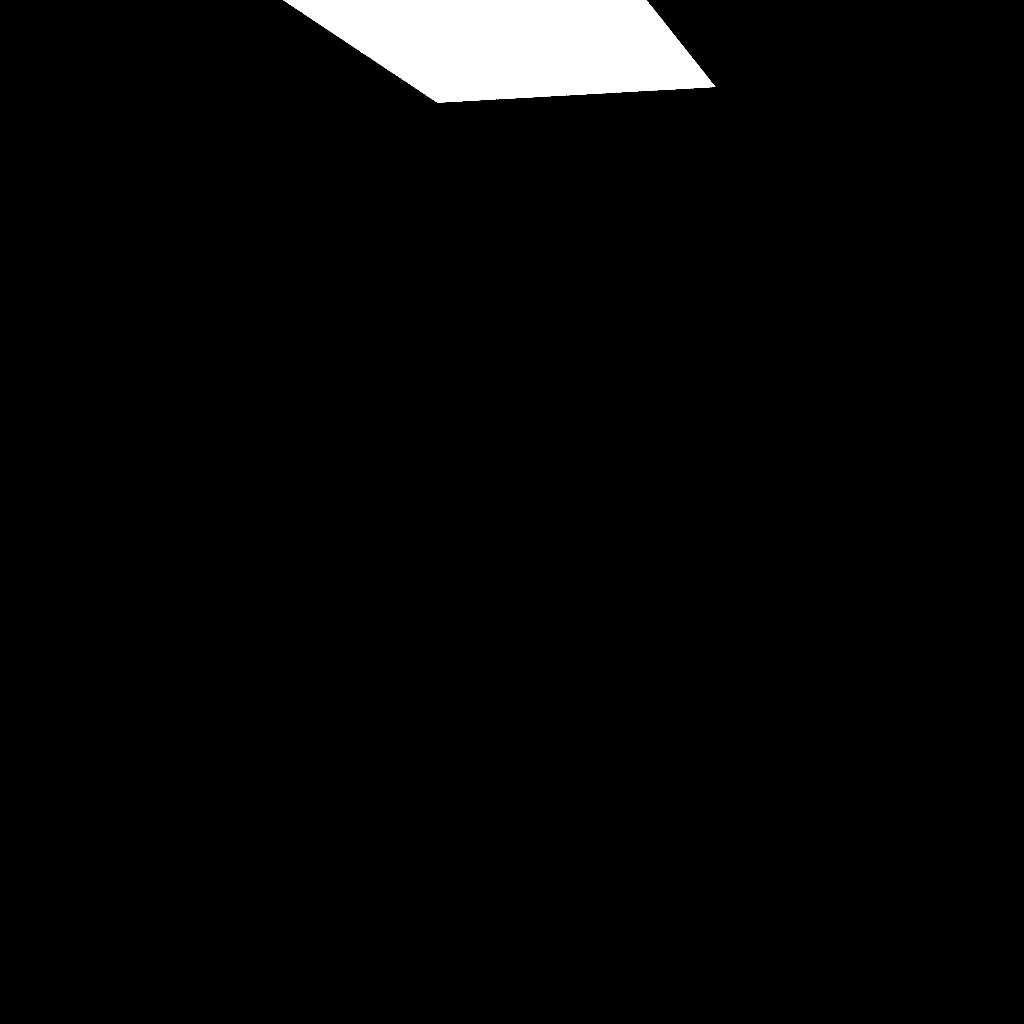
\includegraphics[width=\textwidth]{q2/scene3.png}
      \caption{Rendering of Scene 3}
  \end{minipage}
  \hfill
  \begin{minipage}[t]{.4\textwidth}
      \centering
      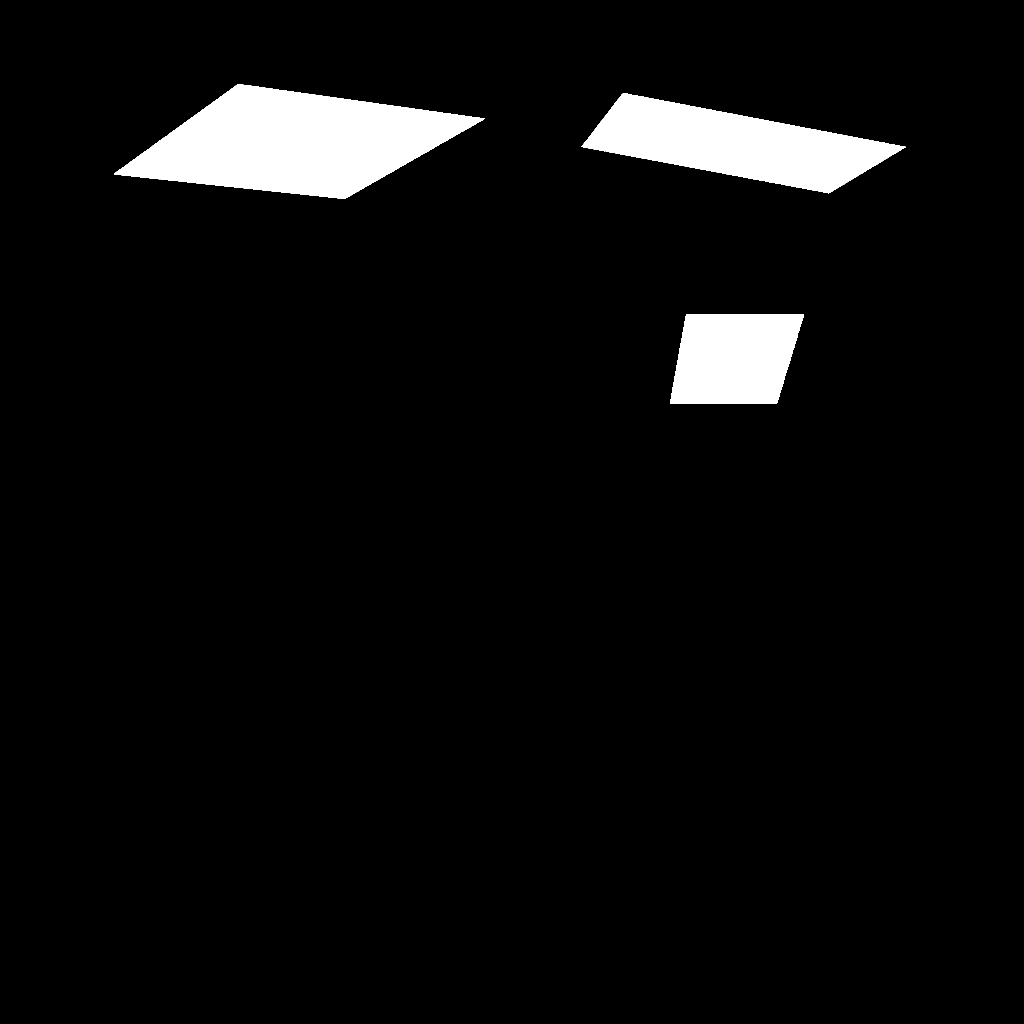
\includegraphics[width=\textwidth]{q2/scene4.png}
      \caption{Rendering of Scene 4}
  \end{minipage}
\end{figure}

\section{Monte-Carlo \& Importance Sampling}

\subsection{Uniform Hemisphere Sampling}

\subsubsection{Timings}

\begin{table}[H]
\centering
\renewcommand{\arraystretch}{1.5}
\begin{tabularx}{\linewidth}{LLL}
\hline
Scene & SPP & Render Time (ms) \\
\hline
\multirow{3}*{Small Area Light} & 10 & 6022.58 \\
                                & 100 & 59144.16 \\
                                & 1000 & 589168.56 \\
\hline
\multirow{3}*{Medium Area Light} & 10 & 6124.01 \\
                                 & 100 & 60336.18 \\
                                 & 1000 & 604133.56 \\
\hline
\multirow{3}*{Big Area Light}   & 10 & 6682.72 \\
                                & 100 & 65333.00 \\
                                & 1000 & 651757.00 \\
\hline
\multirow{3}*{Many Area Lights} & 10 & 8851.31 \\
                                & 100 & 87987.65 \\
                                & 1000 & 874781.50 \\
\hline
\end{tabularx}
\caption{Time taken for rendering models, with Uniform Hemisphere Sampling}
\end{table}

\subsubsection{Rendered Images}

\begin{figure}[H]
  \begin{minipage}[t]{.3\textwidth}
      \centering
      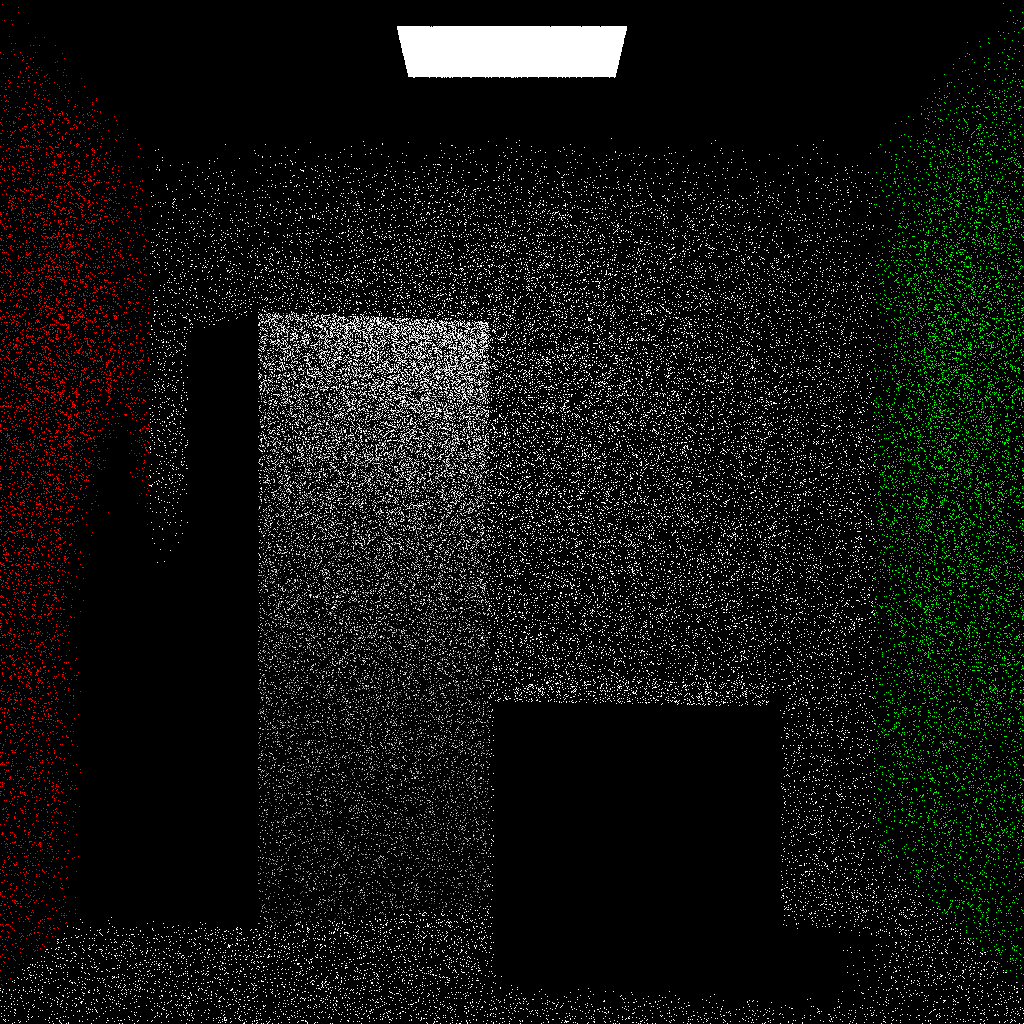
\includegraphics[width=\textwidth]{q3/small_0_10.png}
      \caption{Rendering of Small Area Light, at 10 SPP}
  \end{minipage}
  \hfill
  \begin{minipage}[t]{.3\textwidth}
      \centering
      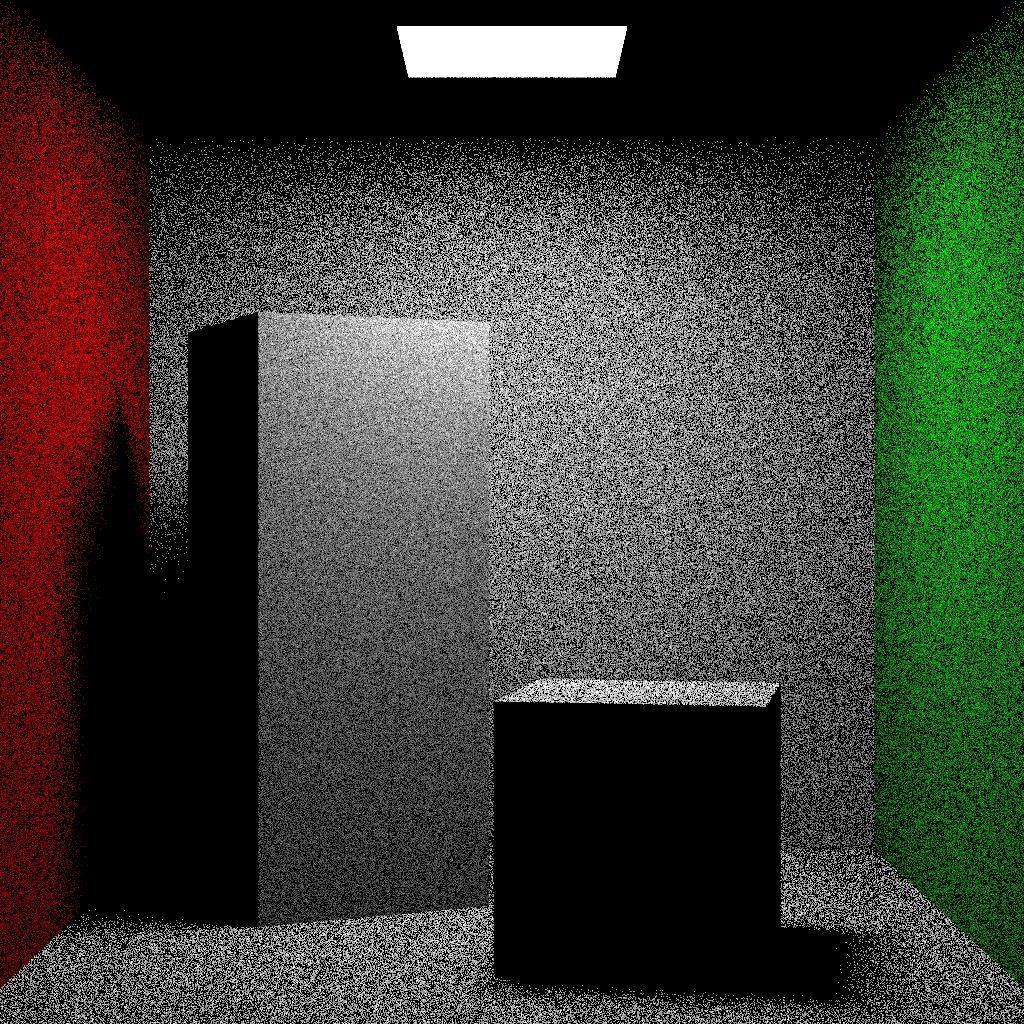
\includegraphics[width=\textwidth]{q3/small_0_100.png}
      \caption{Rendering of Small Area Light, at 100 SPP}
  \end{minipage}
  \hfill
  \begin{minipage}[t]{.3\textwidth}
      \centering
      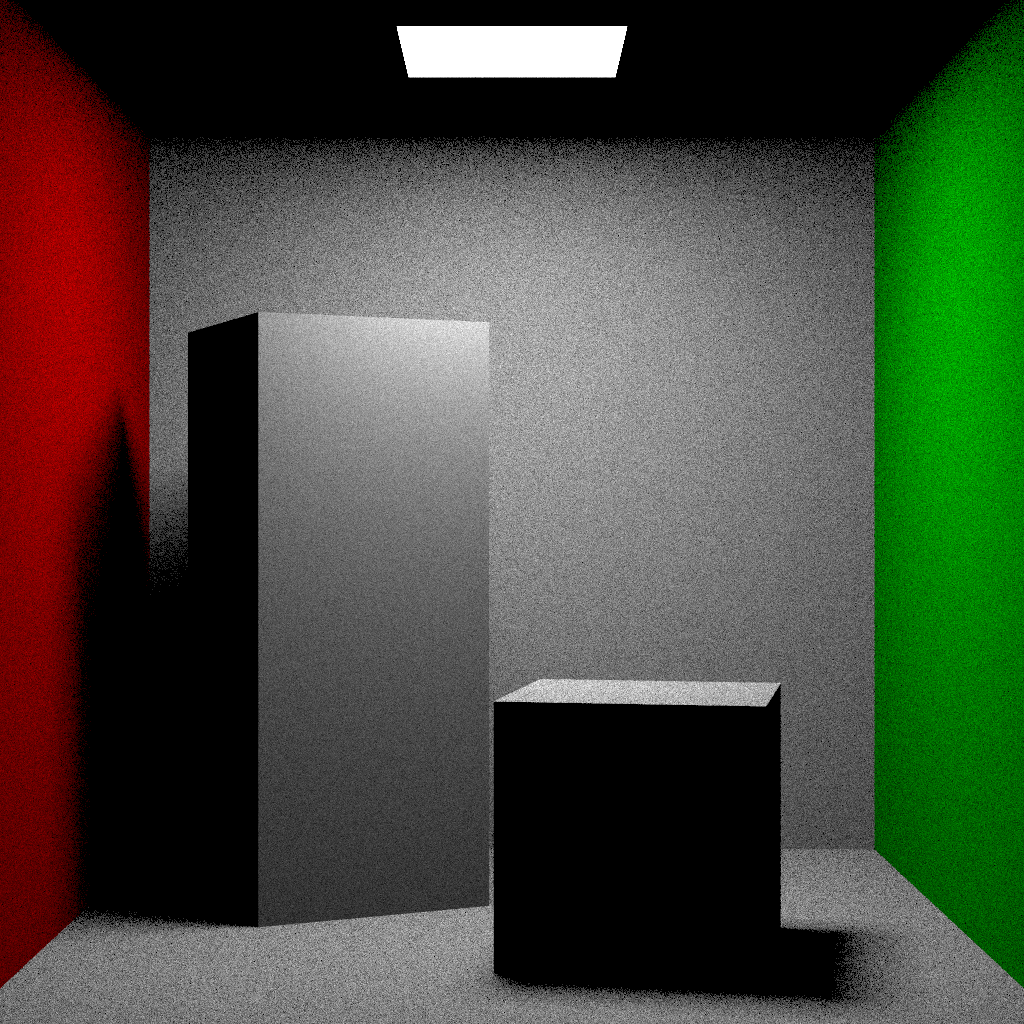
\includegraphics[width=\textwidth]{q3/small_0_1000.png}
      \caption{Rendering of Small Area Light, at 1000 SPP}
  \end{minipage}
\end{figure}

\begin{figure}[H]
  \begin{minipage}[t]{.3\textwidth}
      \centering
      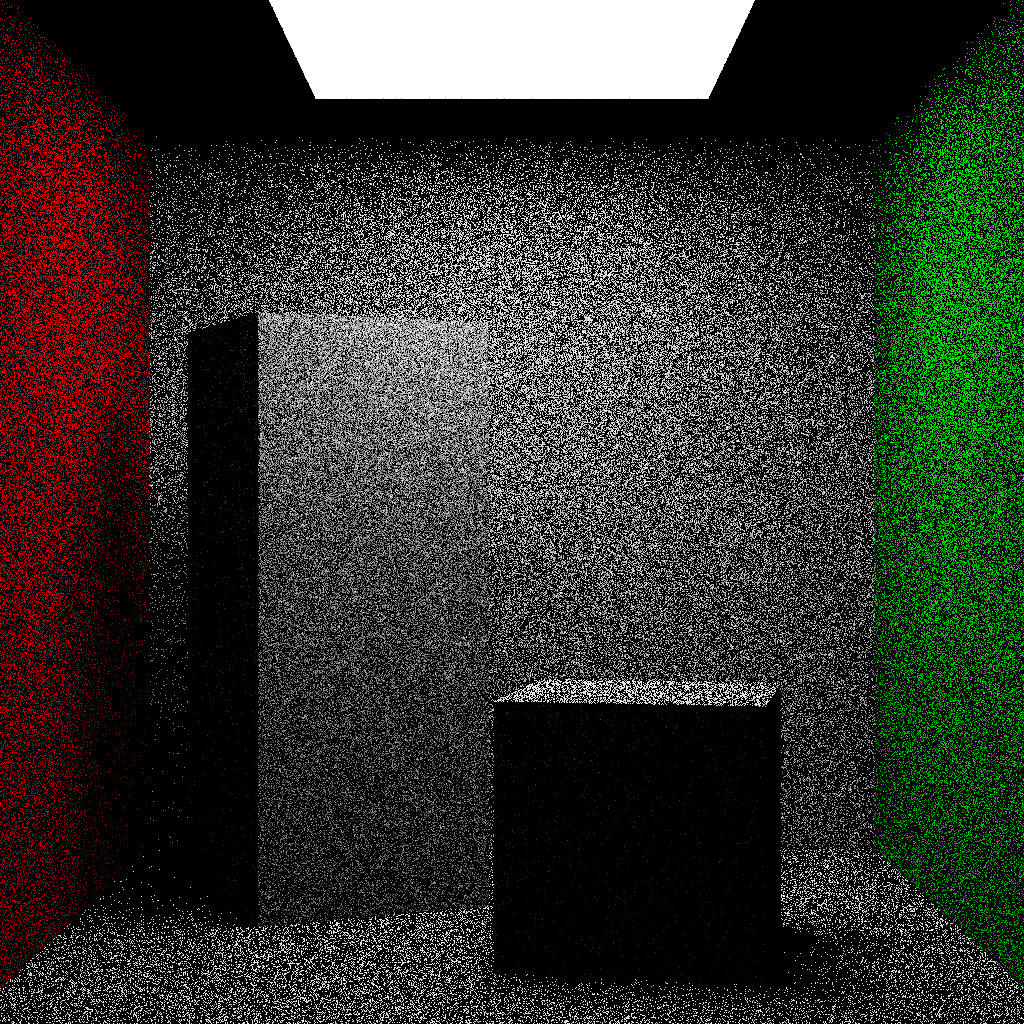
\includegraphics[width=\textwidth]{q3/med_0_10.png}
      \caption{Rendering of Medium Area Light, at 10 SPP}
  \end{minipage}
  \hfill
  \begin{minipage}[t]{.3\textwidth}
      \centering
      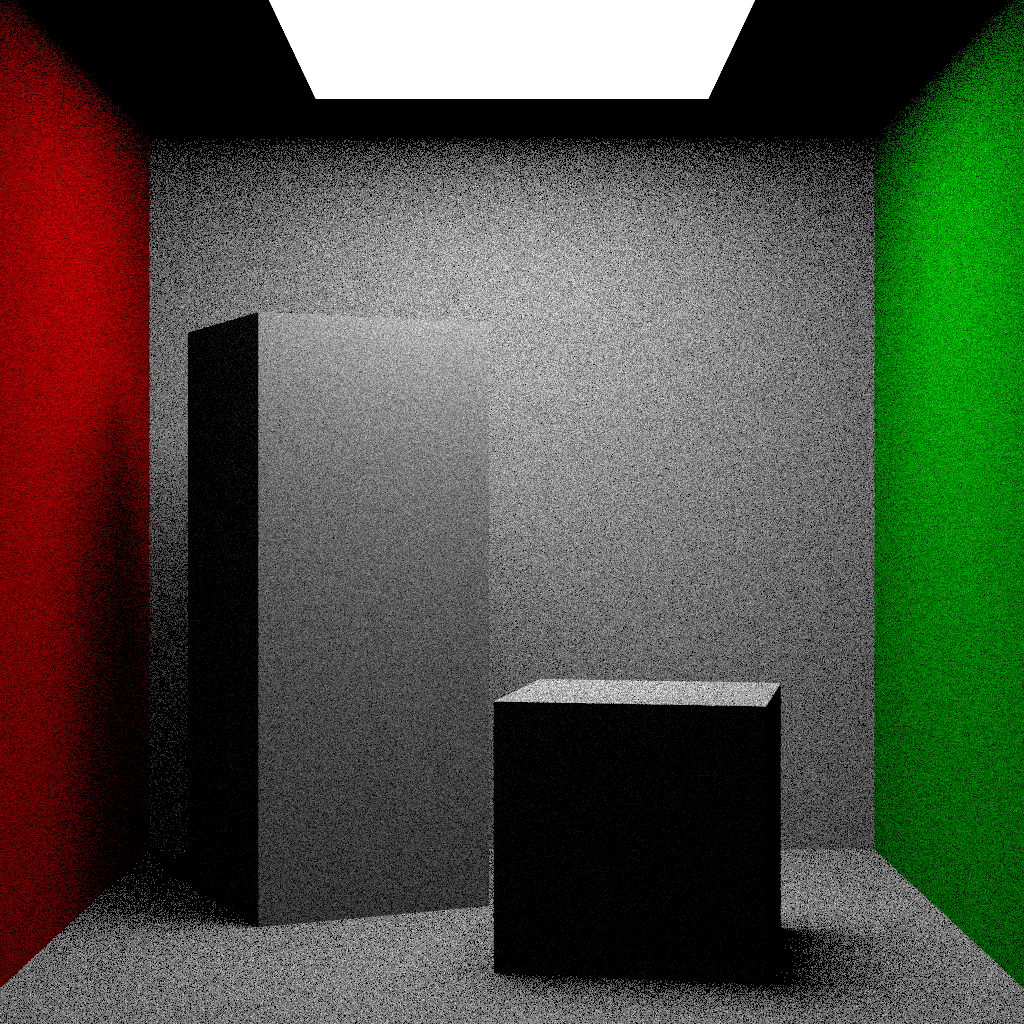
\includegraphics[width=\textwidth]{q3/med_0_100.png}
      \caption{Rendering of Medium Area Light, at 100 SPP}
  \end{minipage}
  \hfill
  \begin{minipage}[t]{.3\textwidth}
      \centering
      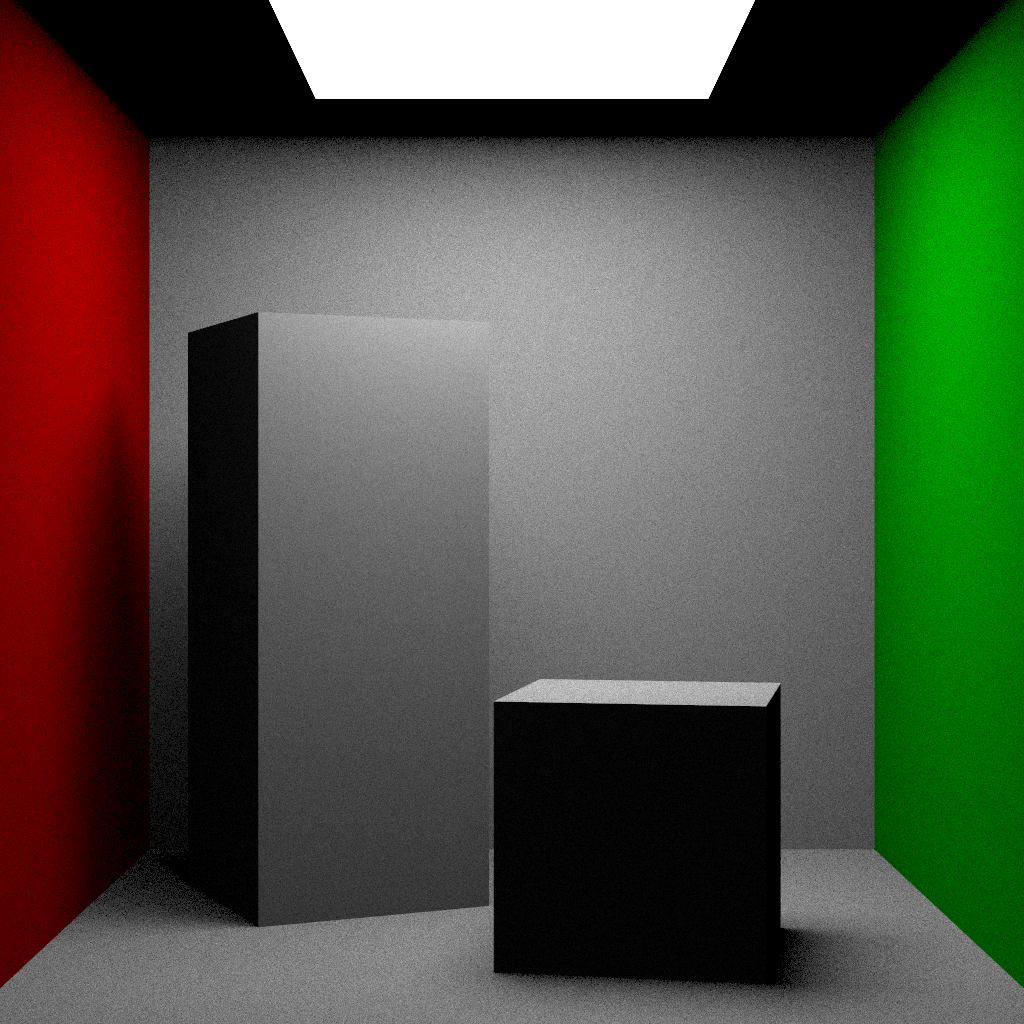
\includegraphics[width=\textwidth]{q3/med_0_1000.png}
      \caption{Rendering of Medium Area Light, at 1000 SPP}
  \end{minipage}
\end{figure}

\begin{figure}[H]
  \begin{minipage}[t]{.3\textwidth}
      \centering
      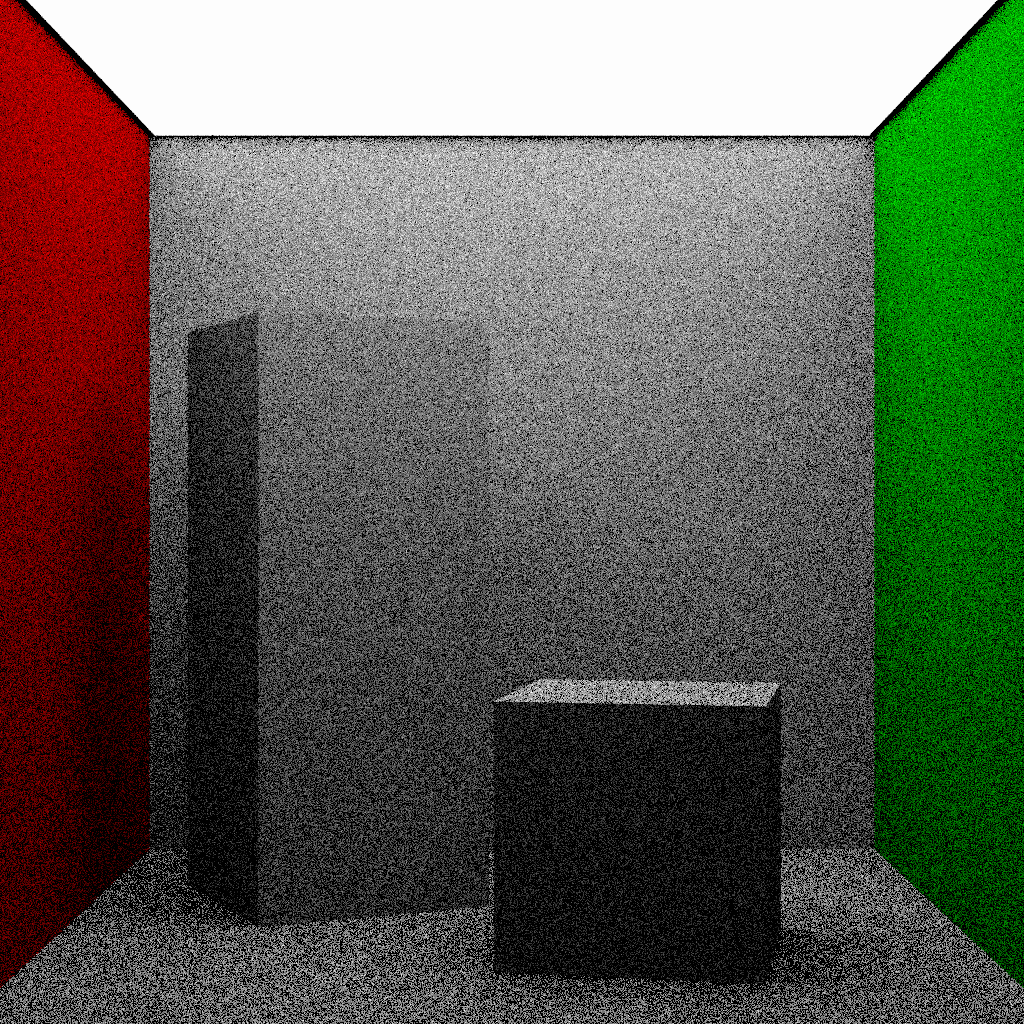
\includegraphics[width=\textwidth]{q3/big_0_10.png}
      \caption{Rendering of Big Area Light, at 10 SPP}
  \end{minipage}
  \hfill
  \begin{minipage}[t]{.3\textwidth}
      \centering
      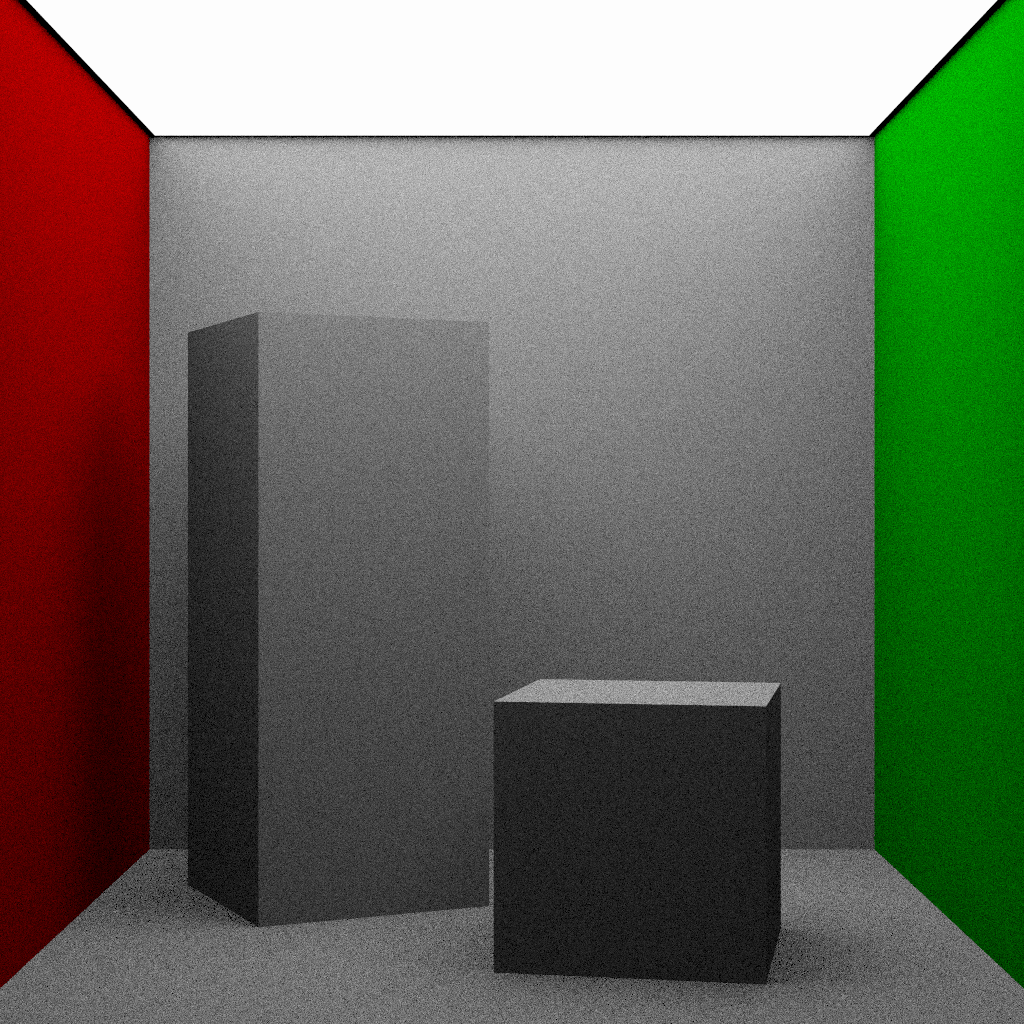
\includegraphics[width=\textwidth]{q3/big_0_100.png}
      \caption{Rendering of Big Area Light, at 100 SPP}
  \end{minipage}
  \hfill
  \begin{minipage}[t]{.3\textwidth}
      \centering
      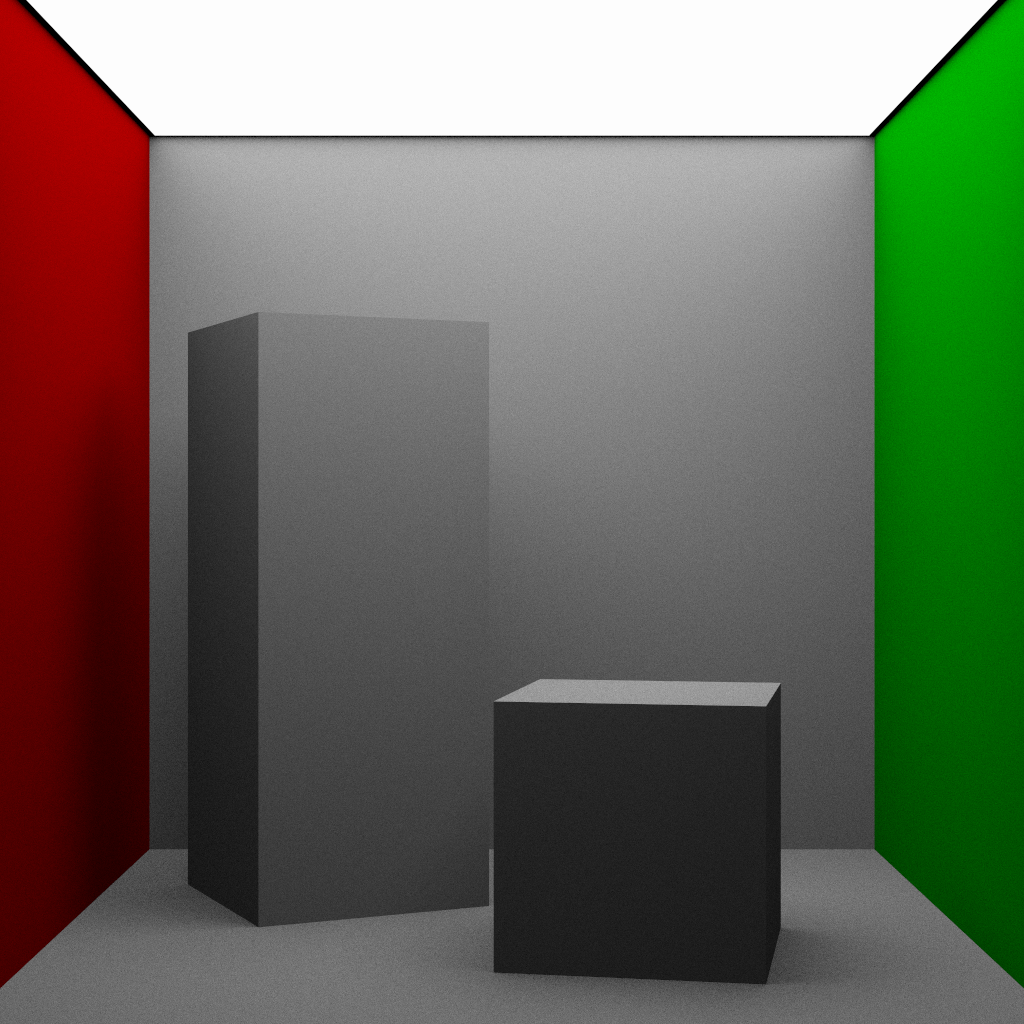
\includegraphics[width=\textwidth]{q3/big_0_1000.png}
      \caption{Rendering of Big Area Light, at 1000 SPP}
  \end{minipage}
\end{figure}

\begin{figure}[H]
  \begin{minipage}[t]{.3\textwidth}
      \centering
      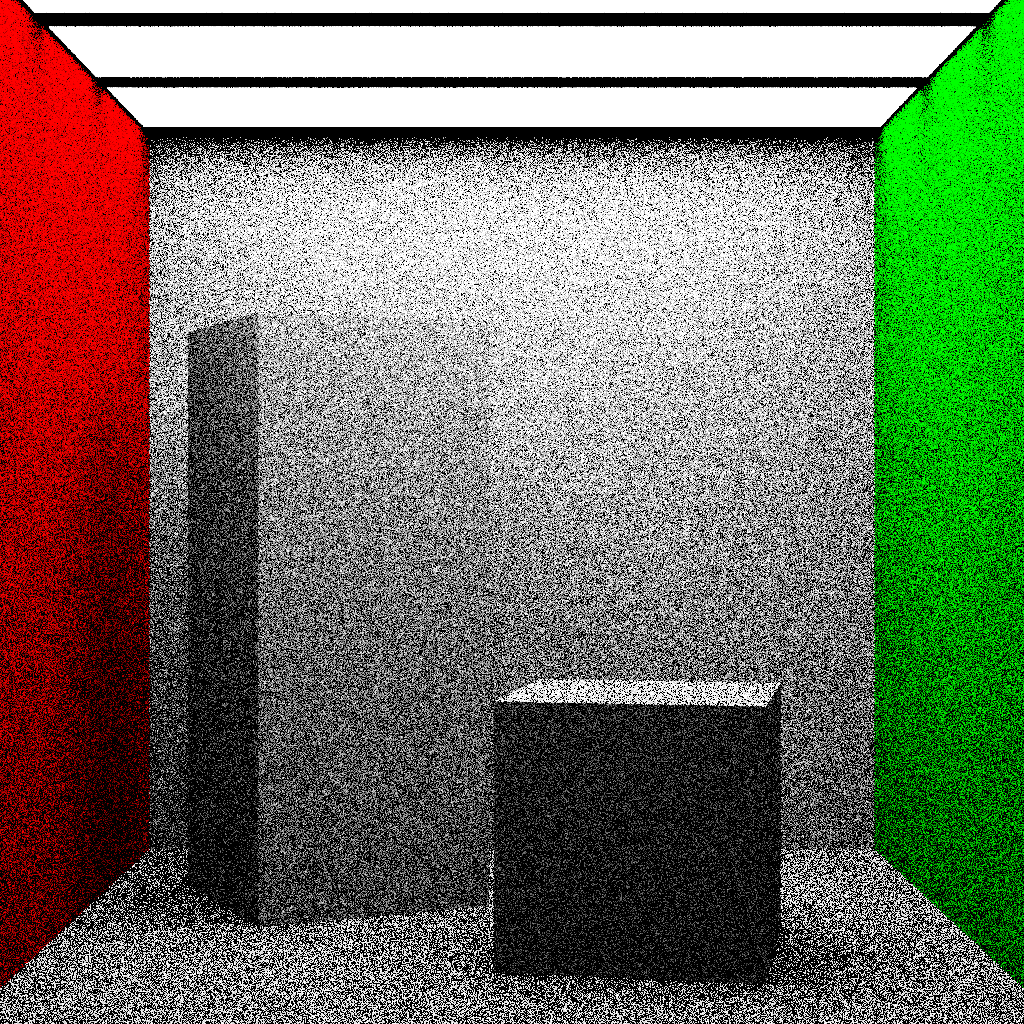
\includegraphics[width=\textwidth]{q3/many_0_10.png}
      \caption{Rendering of Many Area Lights, at 10 SPP}
  \end{minipage}
  \hfill
  \begin{minipage}[t]{.3\textwidth}
      \centering
      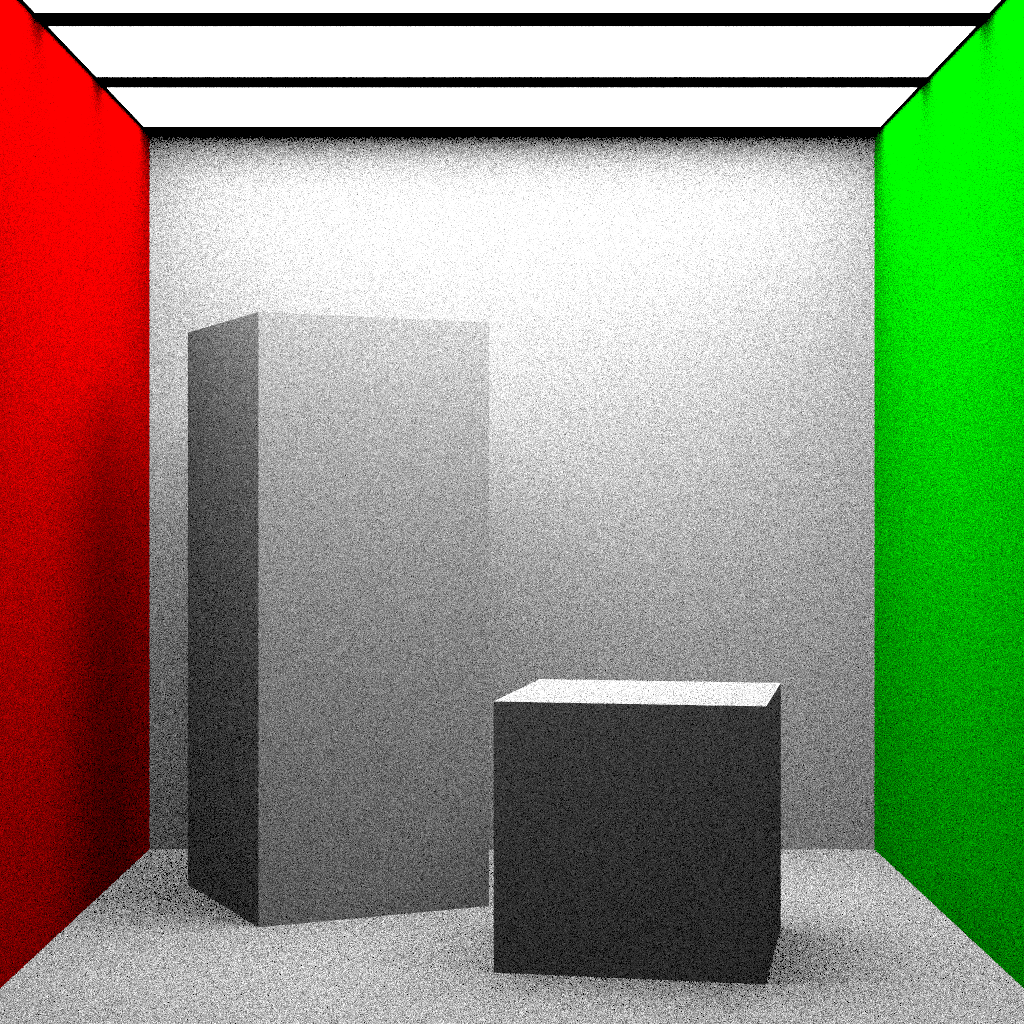
\includegraphics[width=\textwidth]{q3/many_0_100.png}
      \caption{Rendering of Many Area Lights, at 100 SPP}
  \end{minipage}
  \hfill
  \begin{minipage}[t]{.3\textwidth}
      \centering
      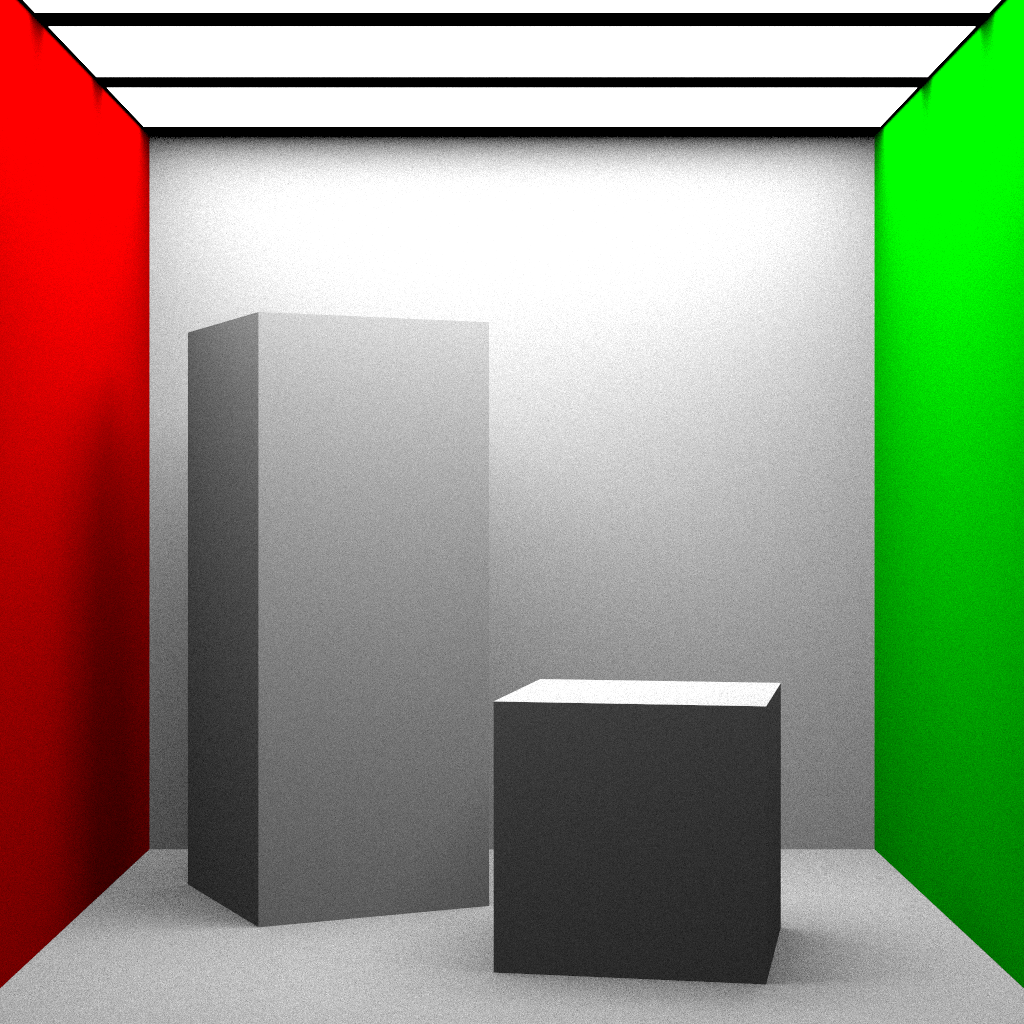
\includegraphics[width=\textwidth]{q3/many_0_1000.png}
      \caption{Rendering of Many Area Lights, at 1000 SPP}
  \end{minipage}
\end{figure}

\subsection{Cosine Weighted Sampling}

\subsubsection{Timings}

\begin{table}[H]
\centering
\renewcommand{\arraystretch}{1.5}
\begin{tabularx}{\linewidth}{LLL}
\hline
Scene & SPP & Render Time (ms) \\
\hline
\multirow{3}*{Small Area Light} & 10 & 6036.33 \\
                                & 100 & 59582.02 \\
                                & 1000 & 592307.38 \\
\hline
\multirow{3}*{Medium Area Light} & 10 & 6207.46 \\
                                 & 100 & 60797.05 \\
                                 & 1000 & 605032.50 \\
\hline
\multirow{3}*{Big Area Light}   & 10 & 6633.85 \\
                                & 100 & 65366.50 \\
                                & 1000 & 651788.44 \\
\hline
\multirow{3}*{Many Area Lights} & 10 & 8912.70 \\
                                & 100 & 90106.61 \\
                                & 1000 & 888110.00 \\
\hline
\end{tabularx}
\caption{Time taken for rendering models, with Cosine Weighted Sampling}
\end{table}

\subsubsection{Rendered Images}

\begin{figure}[H]
  \begin{minipage}[t]{.3\textwidth}
      \centering
      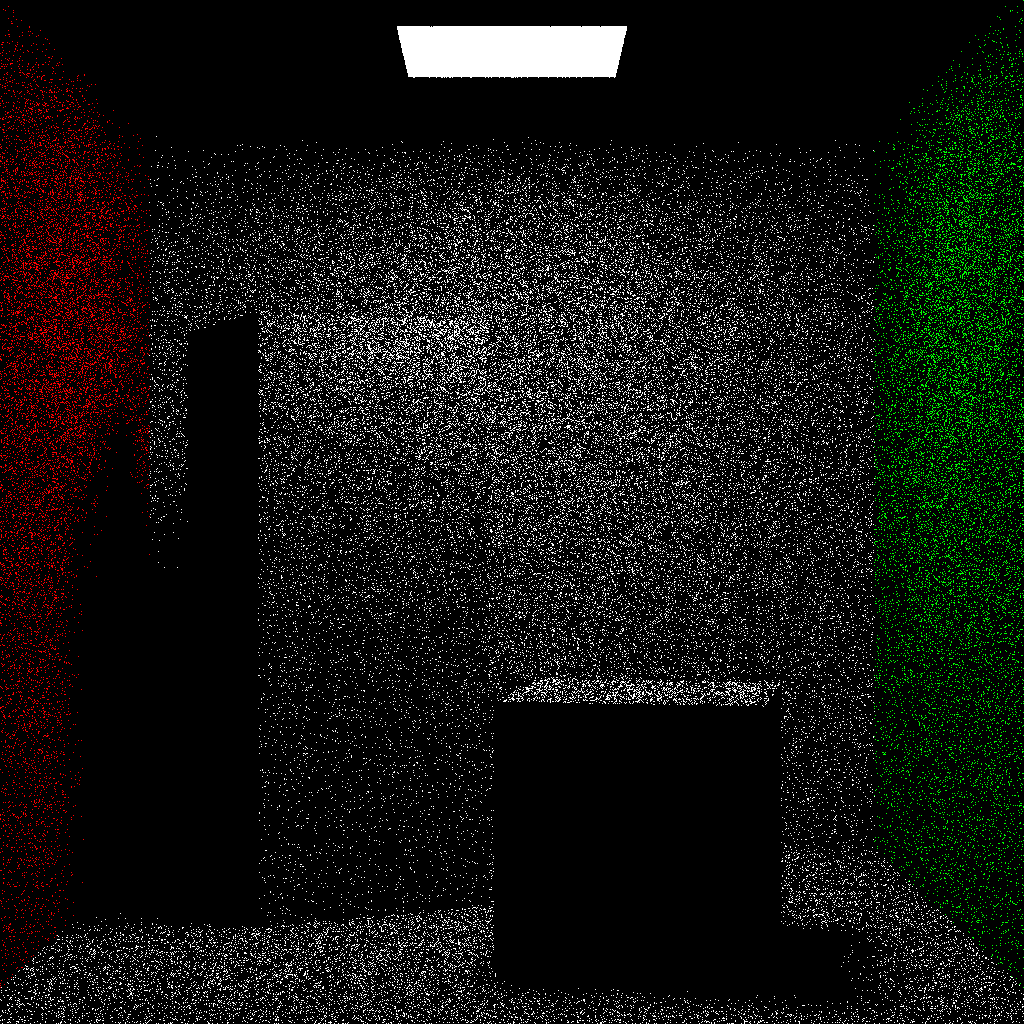
\includegraphics[width=\textwidth]{q3/small_1_10.png}
      \caption{Rendering of Small Area Light, at 10 SPP}
  \end{minipage}
  \hfill
  \begin{minipage}[t]{.3\textwidth}
      \centering
      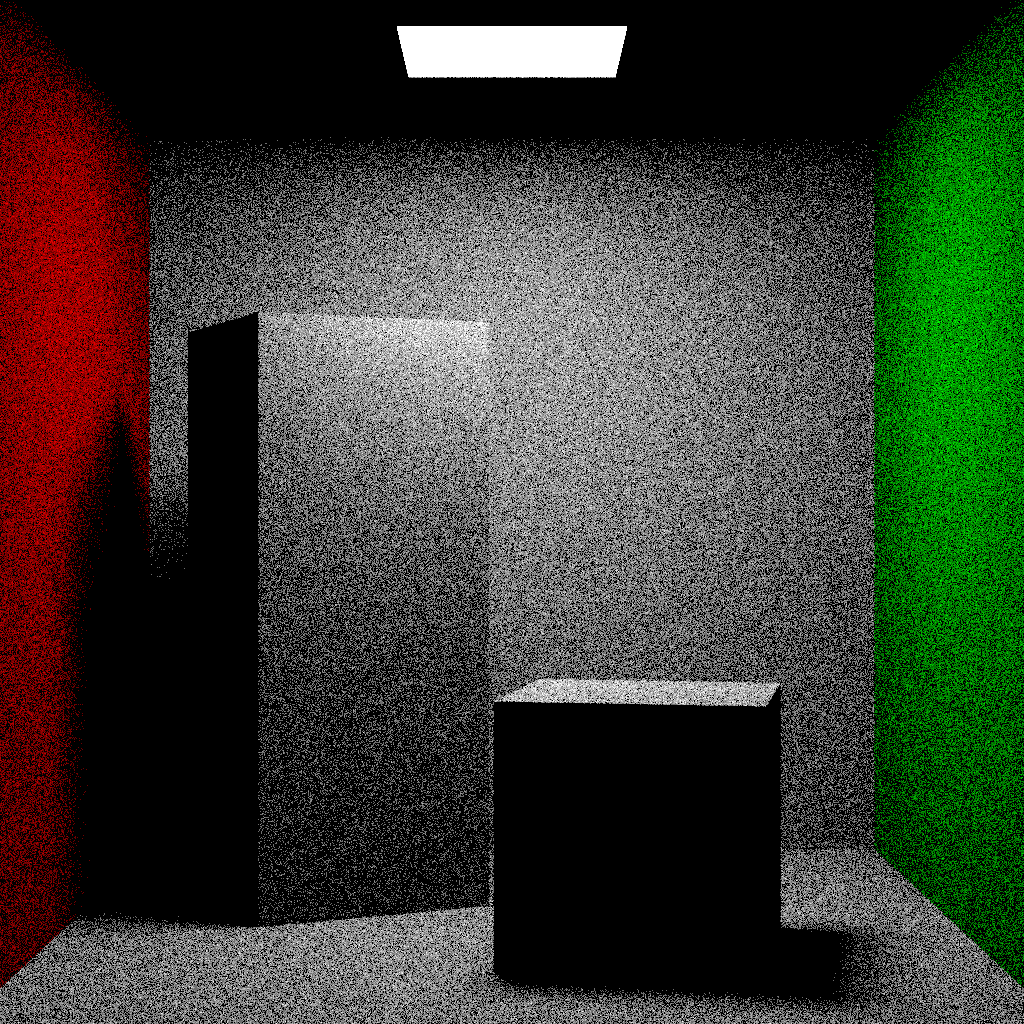
\includegraphics[width=\textwidth]{q3/small_1_100.png}
      \caption{Rendering of Small Area Light, at 100 SPP}
  \end{minipage}
  \hfill
  \begin{minipage}[t]{.3\textwidth}
      \centering
      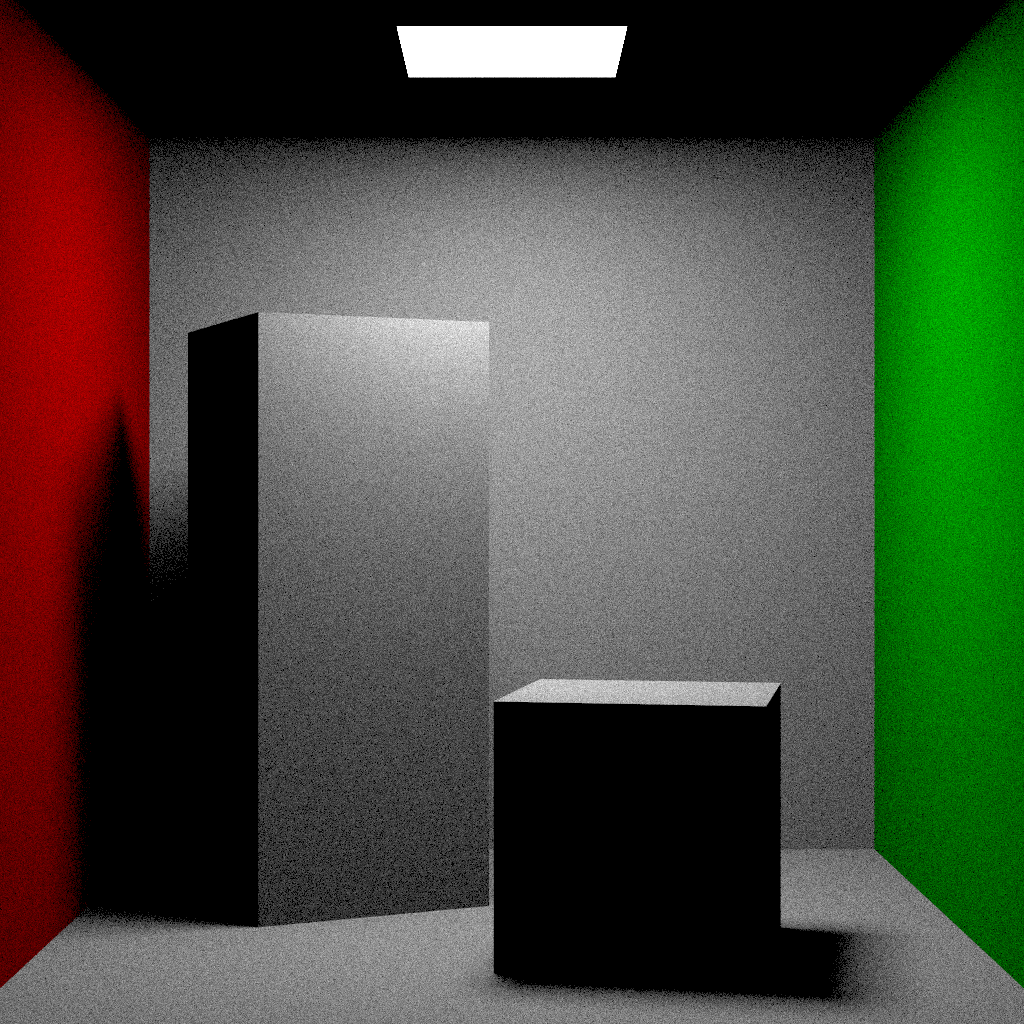
\includegraphics[width=\textwidth]{q3/small_1_1000.png}
      \caption{Rendering of Small Area Light, at 1000 SPP}
  \end{minipage}
\end{figure}

\begin{figure}[H]
  \begin{minipage}[t]{.3\textwidth}
      \centering
      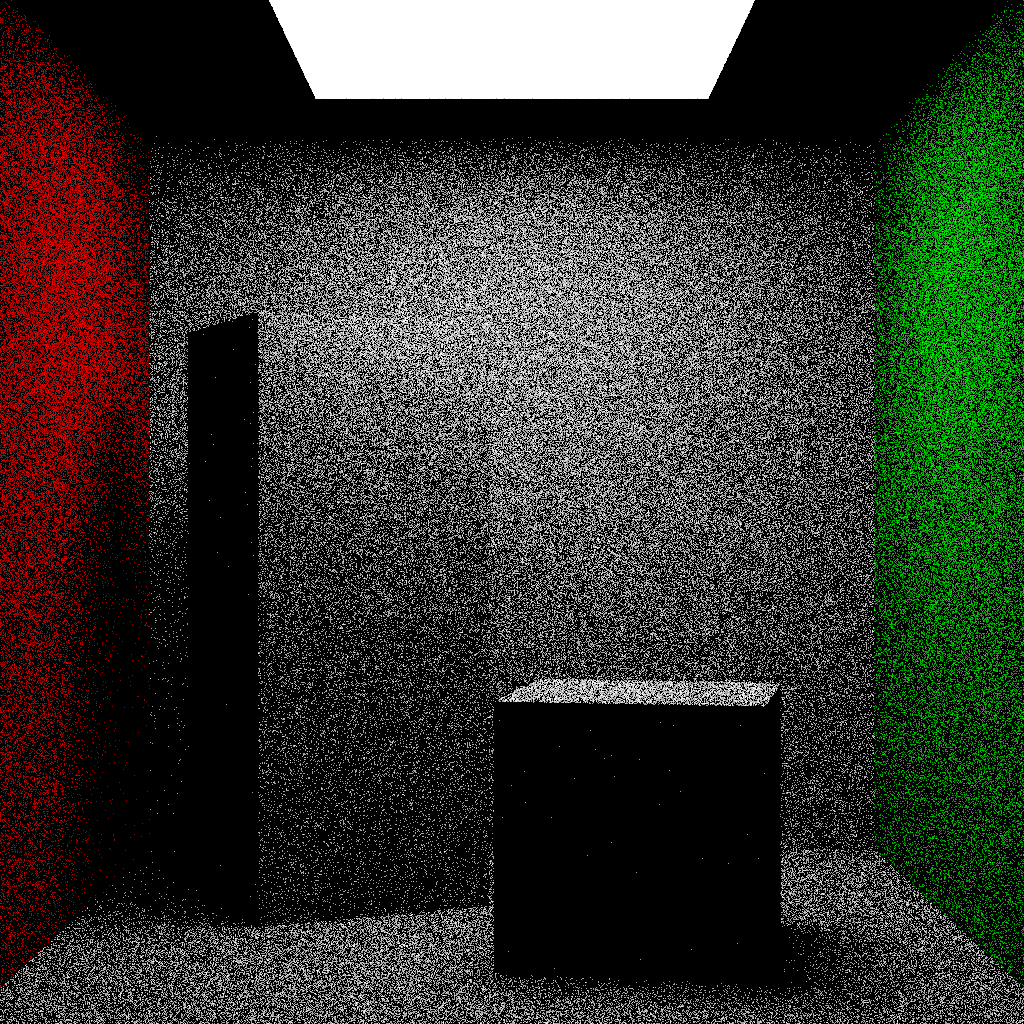
\includegraphics[width=\textwidth]{q3/med_1_10.png}
      \caption{Rendering of Medium Area Light, at 10 SPP}
  \end{minipage}
  \hfill
  \begin{minipage}[t]{.3\textwidth}
      \centering
      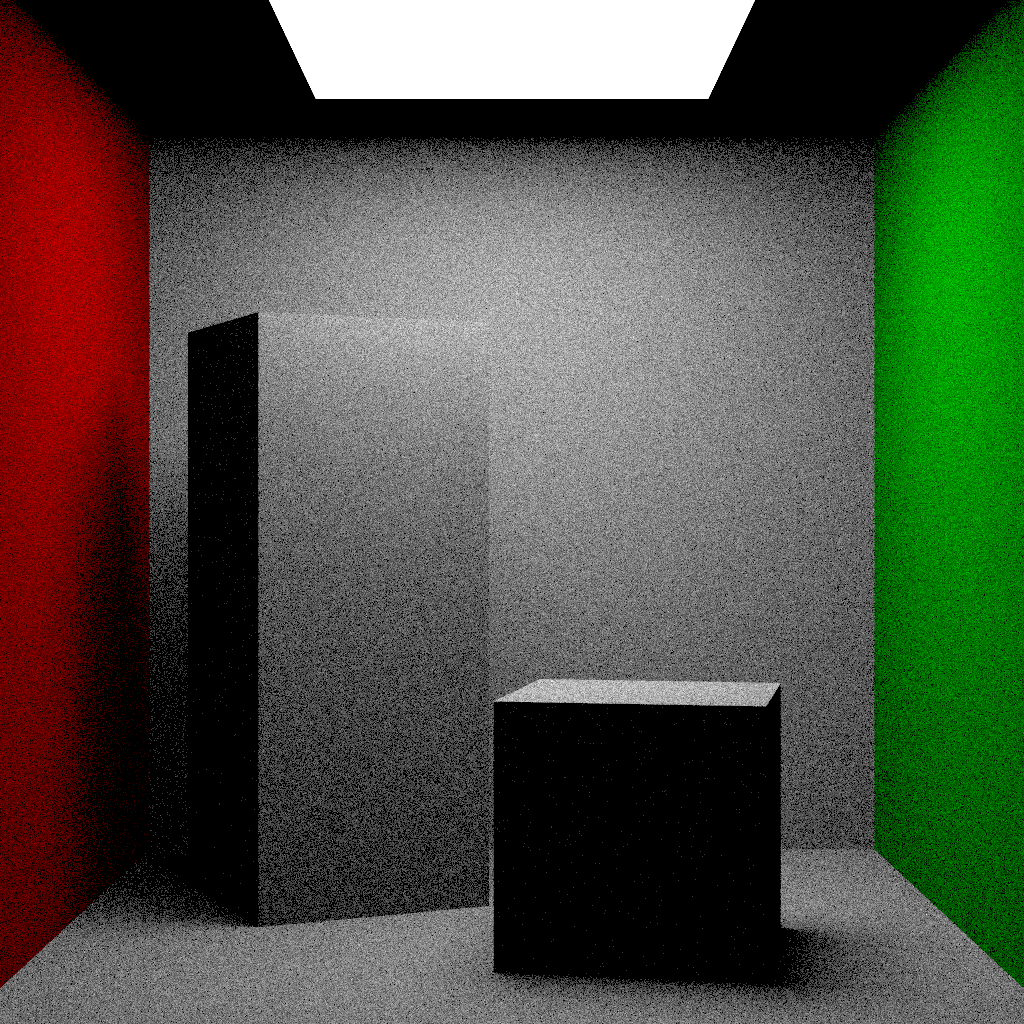
\includegraphics[width=\textwidth]{q3/med_1_100.png}
      \caption{Rendering of Medium Area Light, at 100 SPP}
  \end{minipage}
  \hfill
  \begin{minipage}[t]{.3\textwidth}
      \centering
      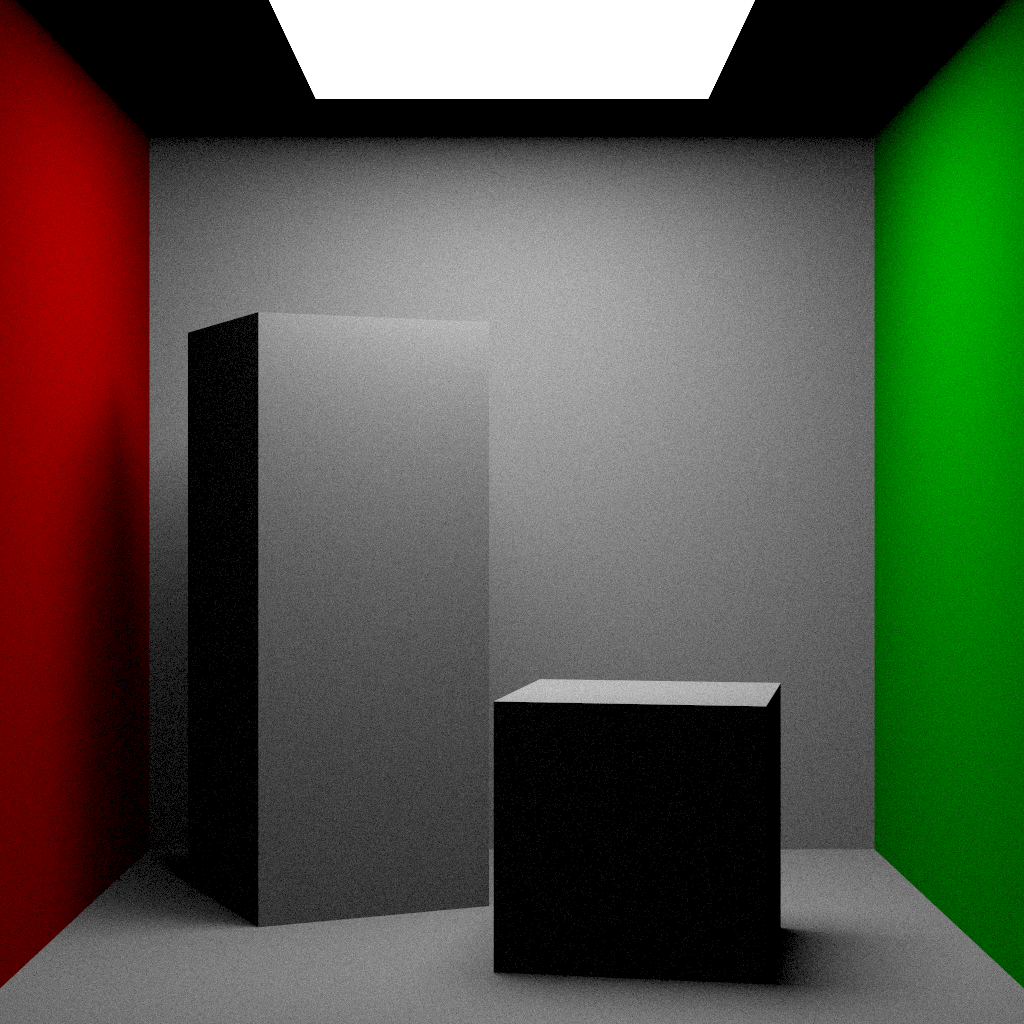
\includegraphics[width=\textwidth]{q3/med_1_1000.png}
      \caption{Rendering of Medium Area Light, at 1000 SPP}
  \end{minipage}
\end{figure}

\begin{figure}[H]
  \begin{minipage}[t]{.3\textwidth}
      \centering
      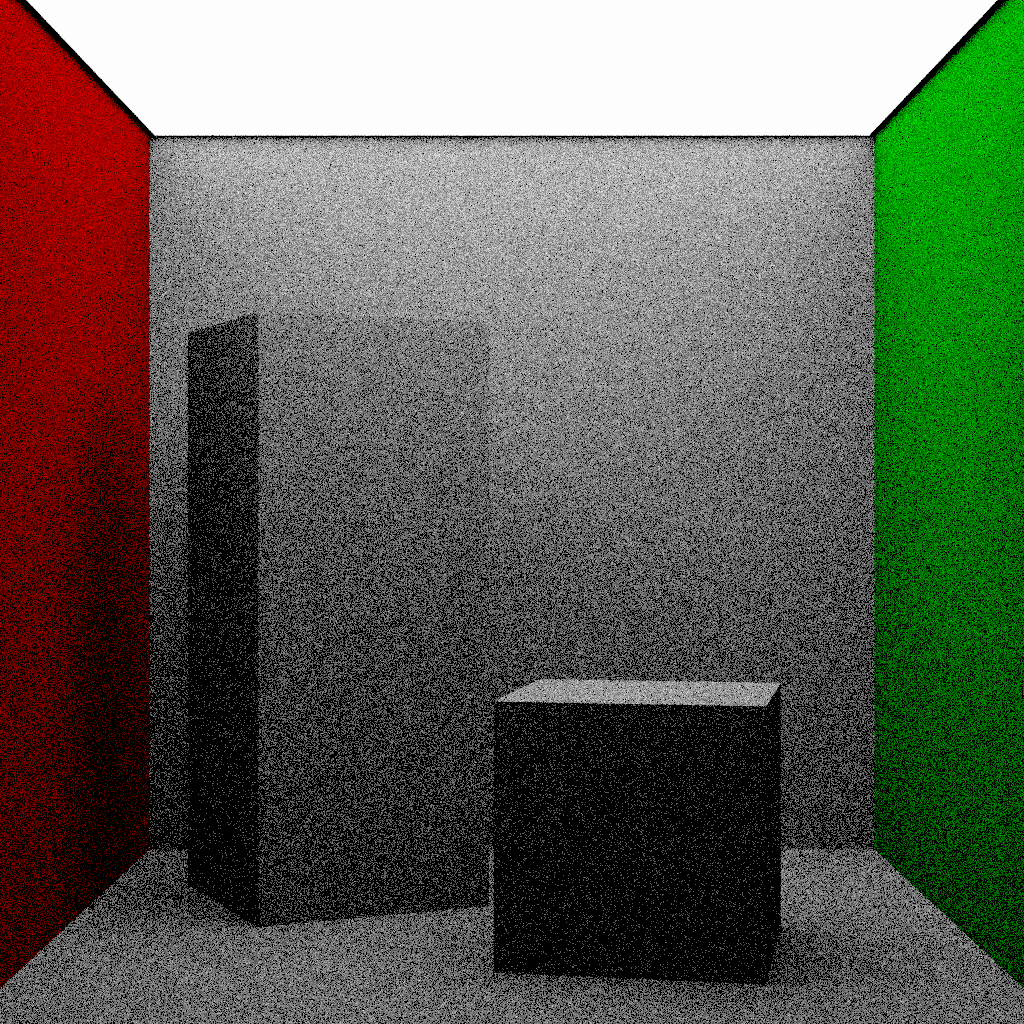
\includegraphics[width=\textwidth]{q3/big_1_10.png}
      \caption{Rendering of Big Area Light, at 10 SPP}
  \end{minipage}
  \hfill
  \begin{minipage}[t]{.3\textwidth}
      \centering
      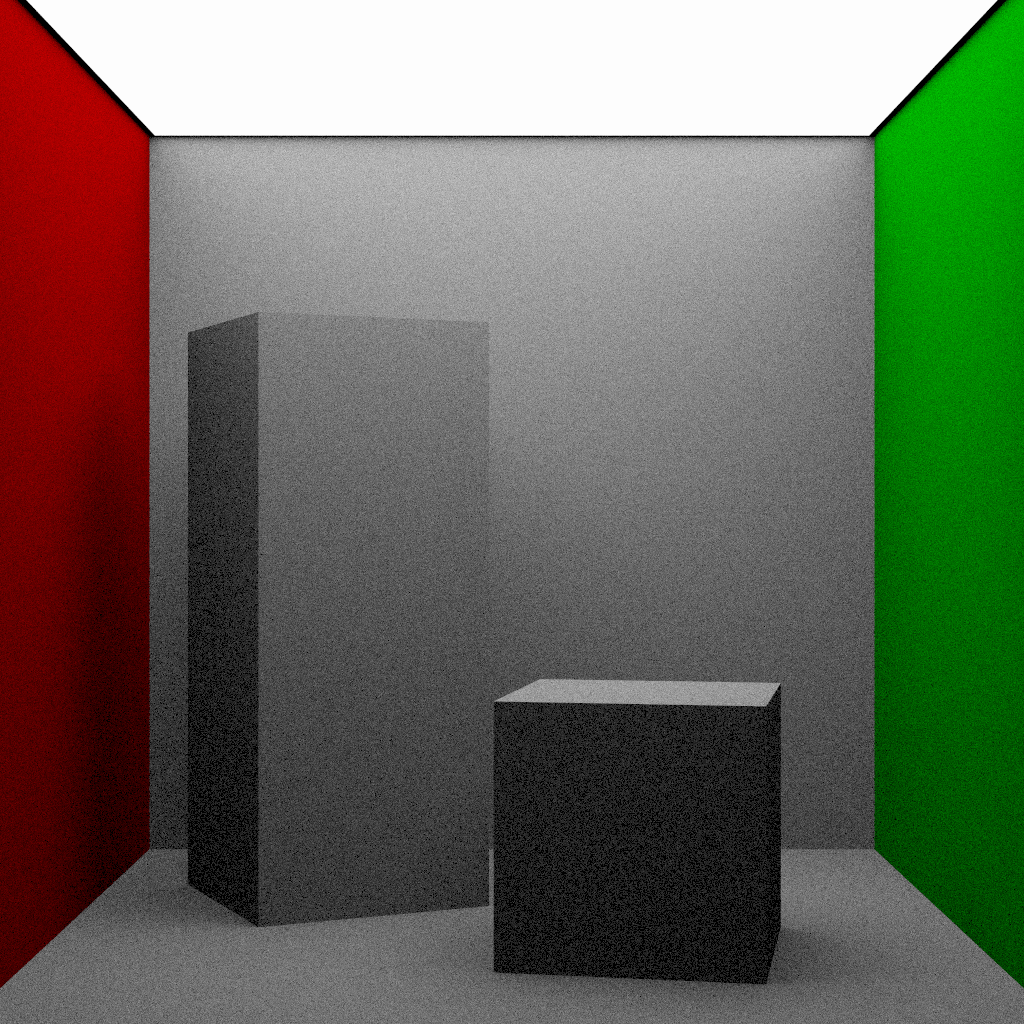
\includegraphics[width=\textwidth]{q3/big_1_100.png}
      \caption{Rendering of Big Area Light, at 100 SPP}
  \end{minipage}
  \hfill
  \begin{minipage}[t]{.3\textwidth}
      \centering
      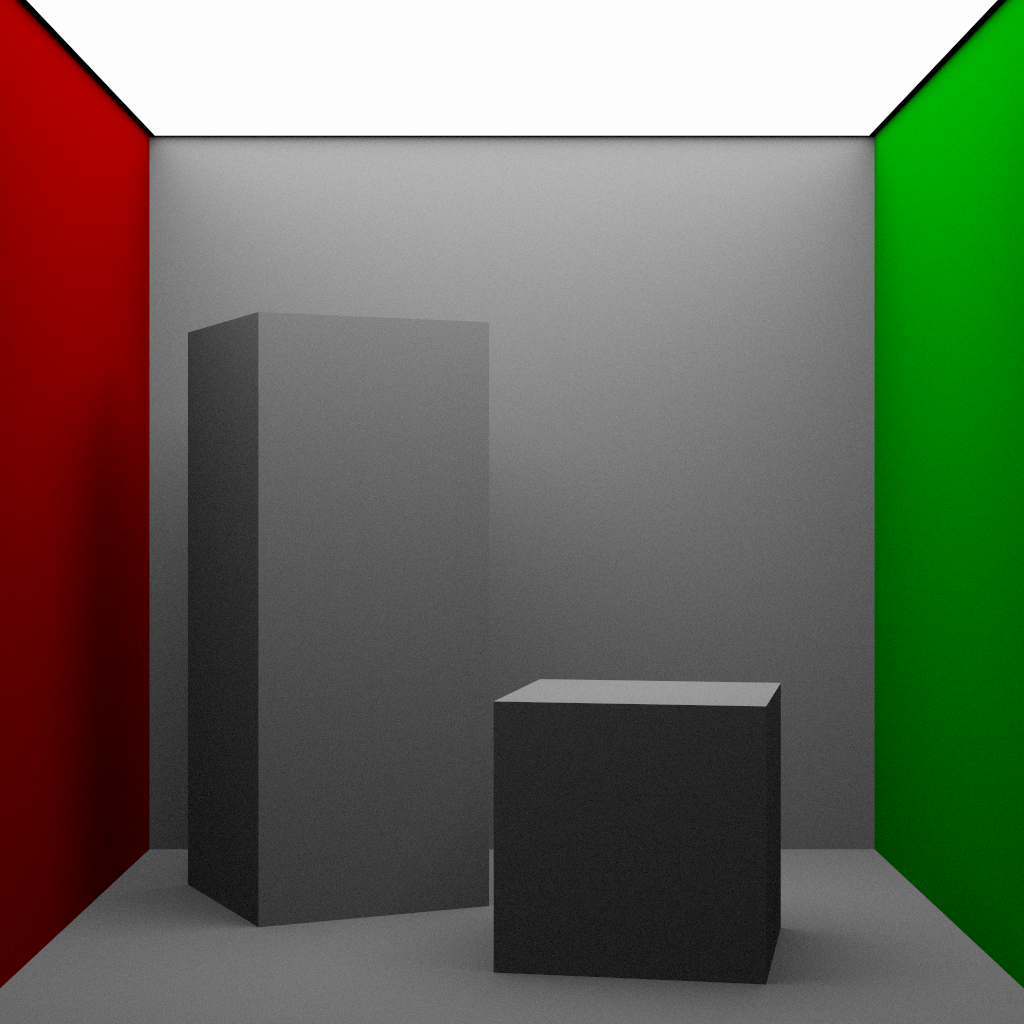
\includegraphics[width=\textwidth]{q3/big_1_1000.png}
      \caption{Rendering of Big Area Light, at 1000 SPP}
  \end{minipage}
\end{figure}

\begin{figure}[H]
  \begin{minipage}[t]{.3\textwidth}
      \centering
      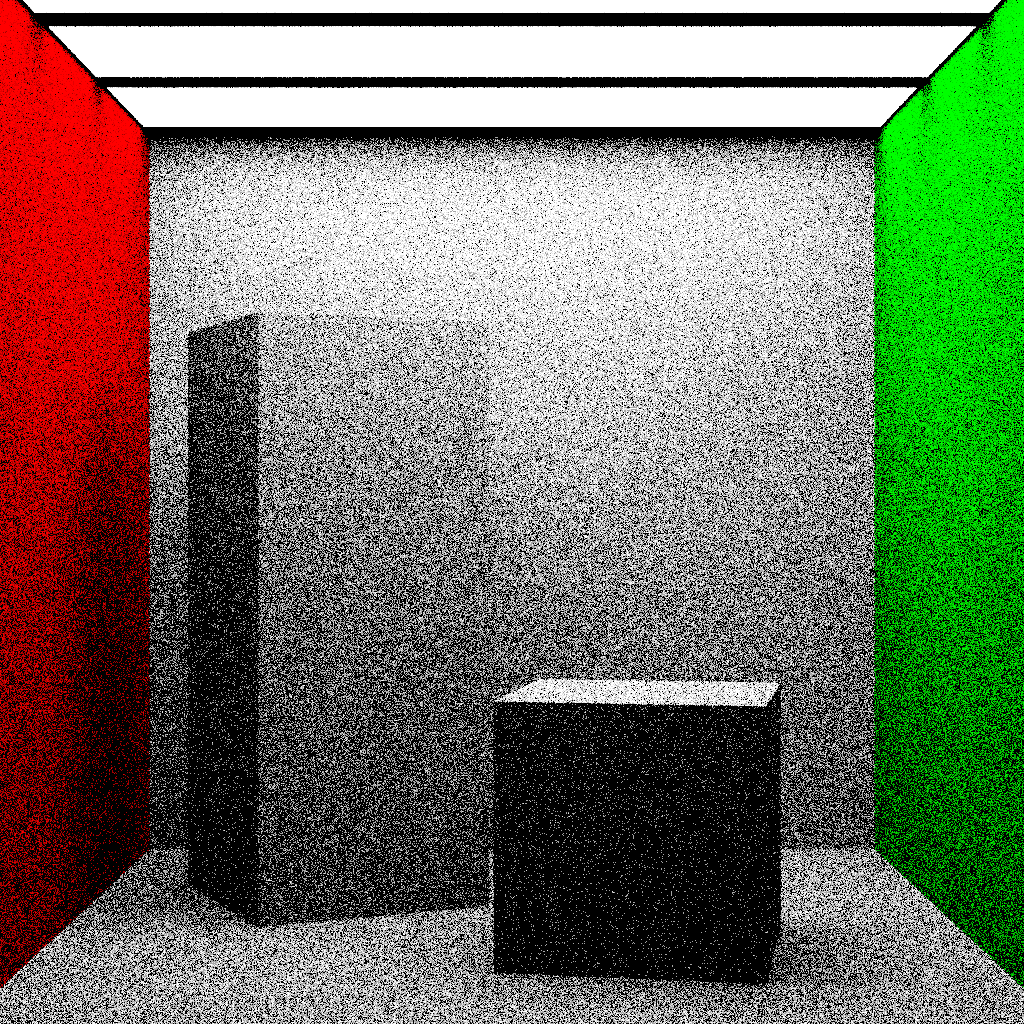
\includegraphics[width=\textwidth]{q3/many_1_10.png}
      \caption{Rendering of Many Area Lights, at 10 SPP}
  \end{minipage}
  \hfill
  \begin{minipage}[t]{.3\textwidth}
      \centering
      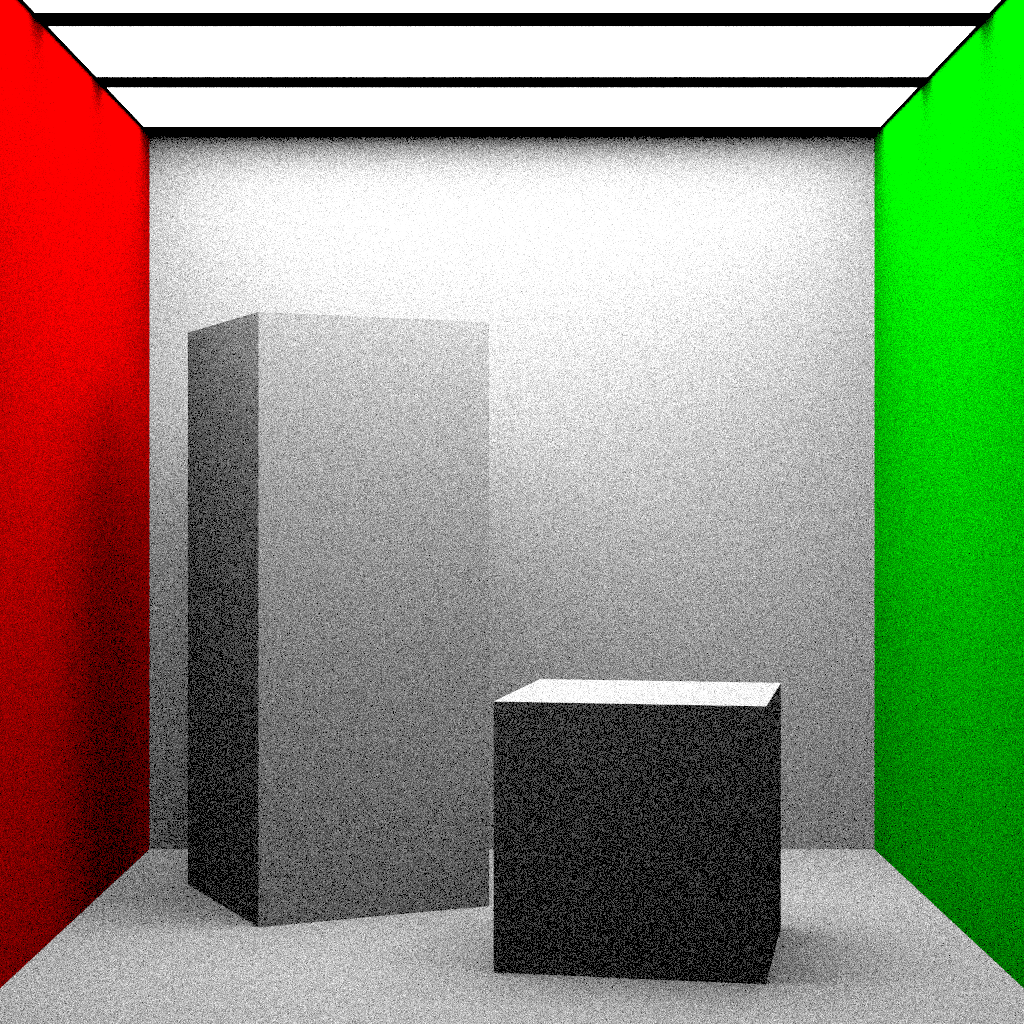
\includegraphics[width=\textwidth]{q3/many_1_100.png}
      \caption{Rendering of Many Area Lights, at 100 SPP}
  \end{minipage}
  \hfill
  \begin{minipage}[t]{.3\textwidth}
      \centering
      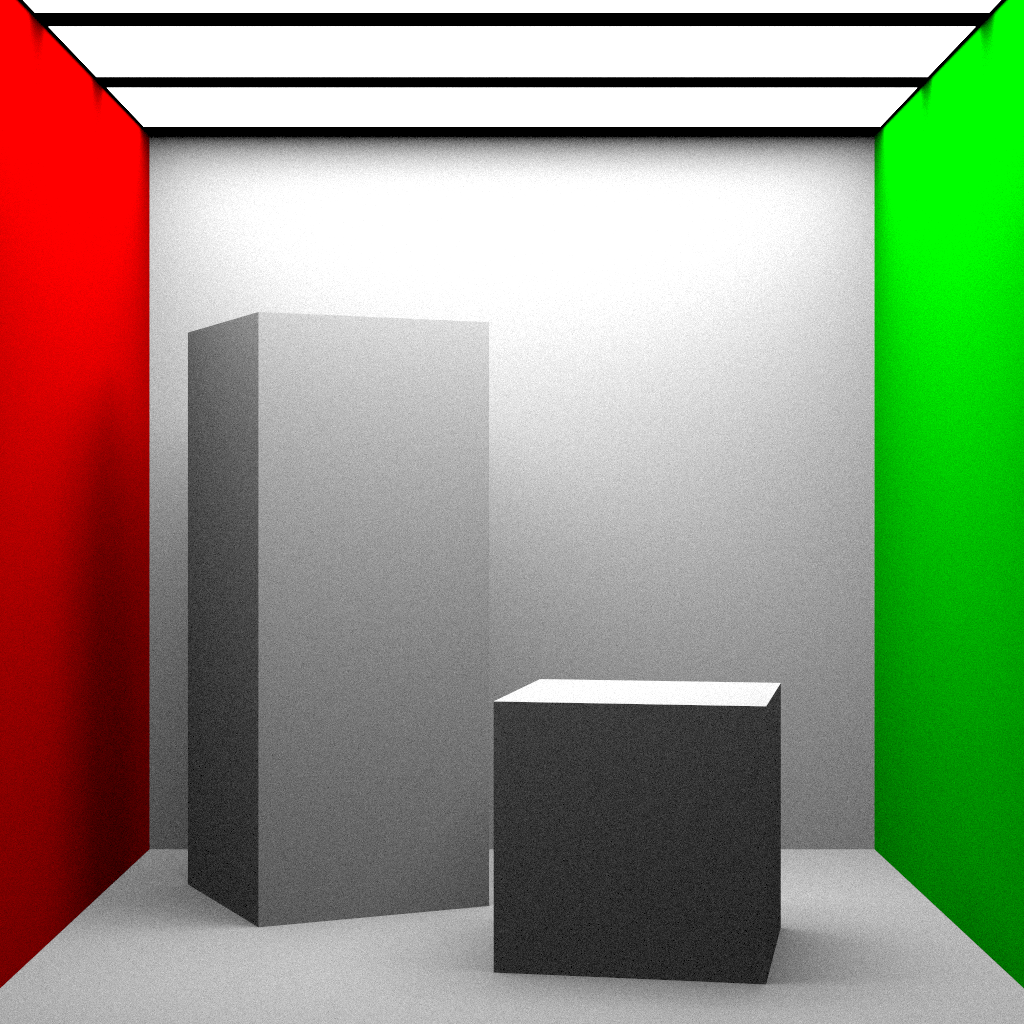
\includegraphics[width=\textwidth]{q3/many_1_1000.png}
      \caption{Rendering of Many Area Lights, at 1000 SPP}
  \end{minipage}
\end{figure}

\subsection{Light Sampling}

\subsubsection{Timings}

\begin{table}[H]
\centering
\renewcommand{\arraystretch}{1.5}
\begin{tabularx}{\linewidth}{LLL}
\hline
Scene & SPP & Render Time (ms) \\
\hline
\multirow{3}*{Small Area Light} & 10 & 9806.28 \\
                                & 100 & 97156.87 \\
                                & 1000 & 971337.81 \\
\hline
\multirow{3}*{Medium Area Light} & 10 & 9932.09 \\
                                 & 100 & 98510.02 \\
                                 & 1000 & 983582.56 \\
\hline
\multirow{3}*{Big Area Light}   & 10 & 10076.54 \\
                                & 100 & 99681.77 \\
                                & 1000 & 996459.94 \\
\hline
\multirow{3}*{Many Area Lights} & 10 & 20799.39 \\
                                & 100 & 205285.19 \\
                                & 1000 & 2048712.50 \\
\hline
\end{tabularx}
\caption{Time taken for rendering models, with Light Sampling}
\end{table}

\subsubsection{Rendered Images}

\begin{figure}[H]
  \begin{minipage}[t]{.3\textwidth}
      \centering
      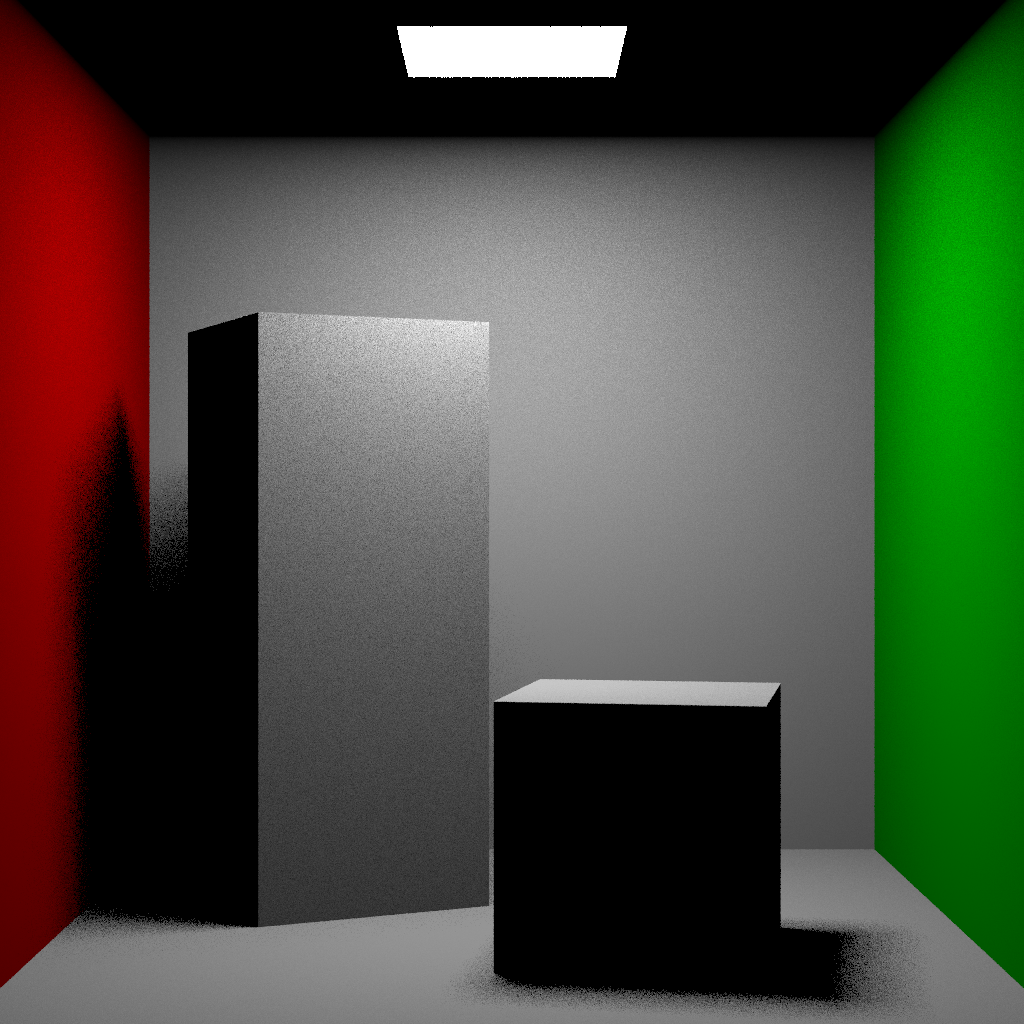
\includegraphics[width=\textwidth]{q3/small_2_10.png}
      \caption{Rendering of Small Area Light, at 10 SPP}
  \end{minipage}
  \hfill
  \begin{minipage}[t]{.3\textwidth}
      \centering
      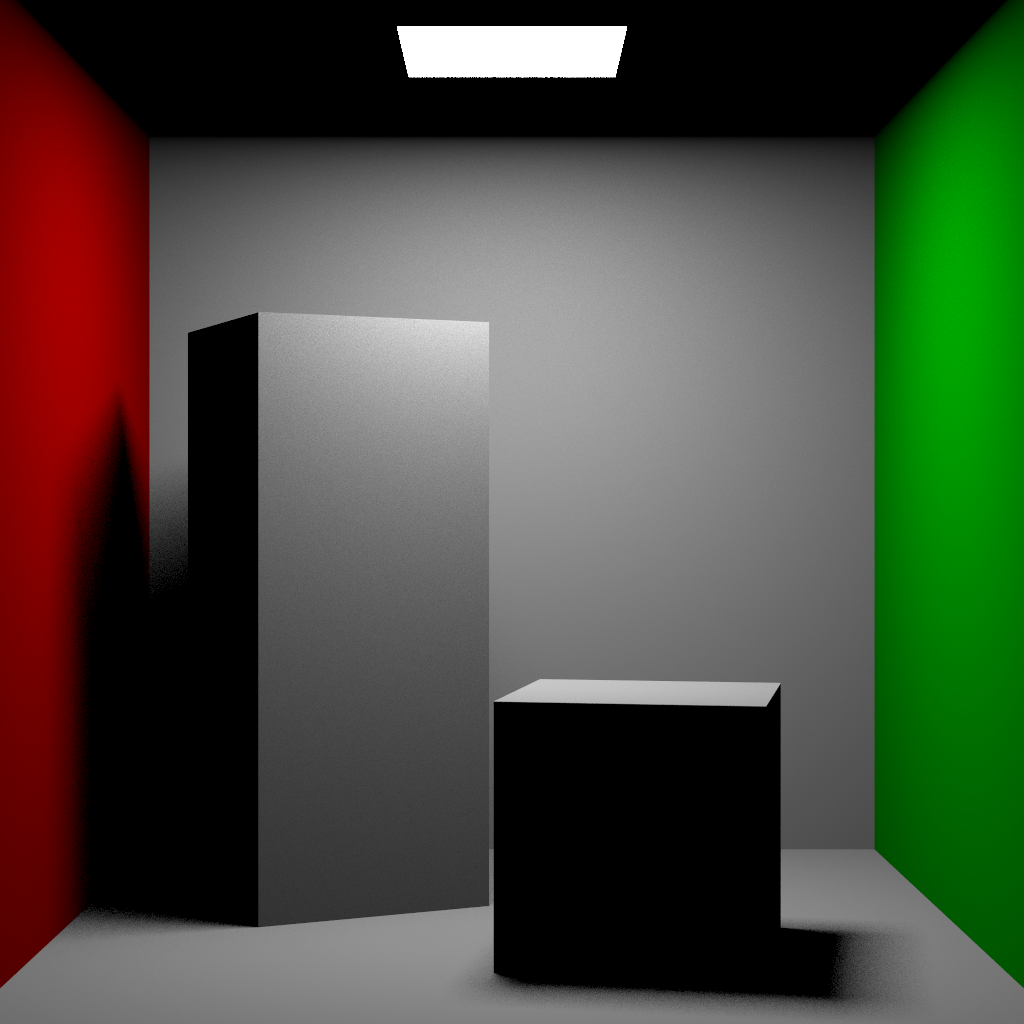
\includegraphics[width=\textwidth]{q3/small_2_100.png}
      \caption{Rendering of Small Area Light, at 100 SPP}
  \end{minipage}
  \hfill
  \begin{minipage}[t]{.3\textwidth}
      \centering
      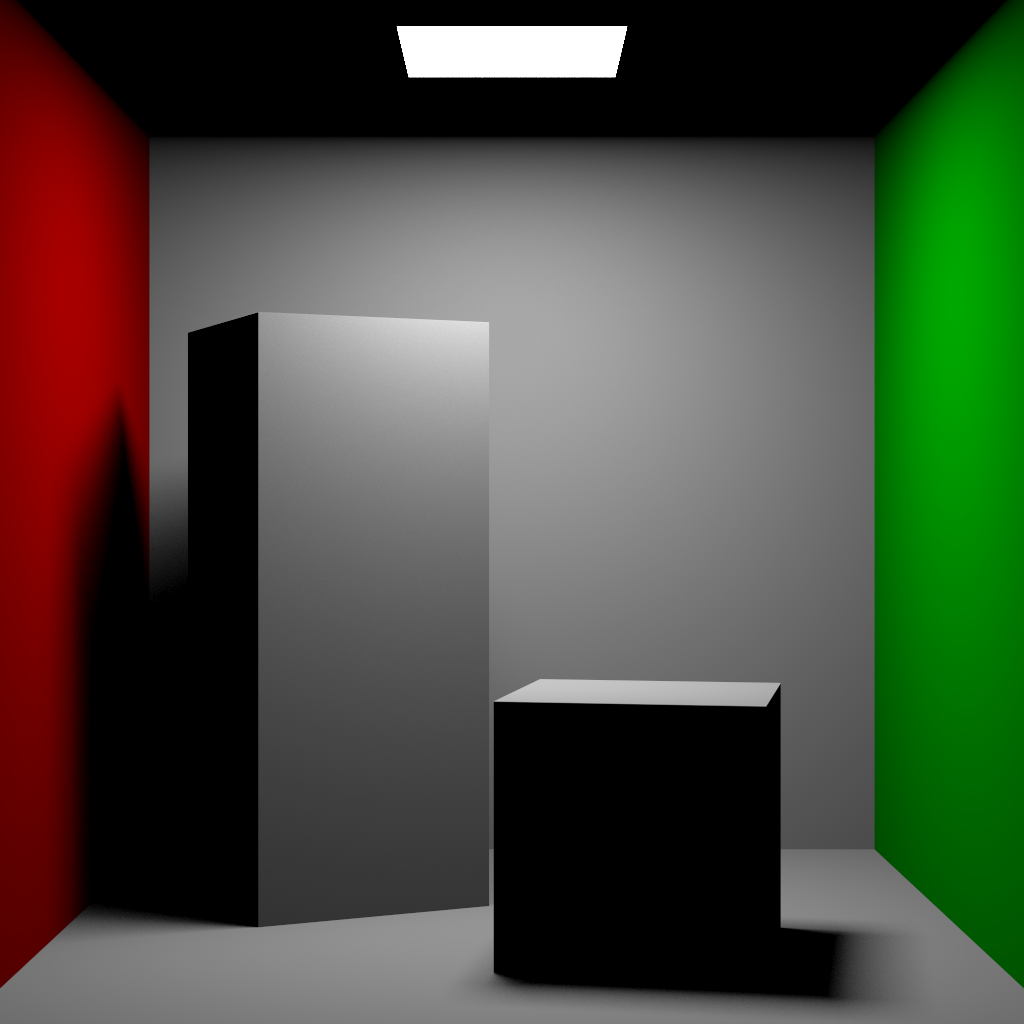
\includegraphics[width=\textwidth]{q3/small_2_1000.png}
      \caption{Rendering of Small Area Light, at 1000 SPP}
  \end{minipage}
\end{figure}

\begin{figure}[H]
  \begin{minipage}[t]{.3\textwidth}
      \centering
      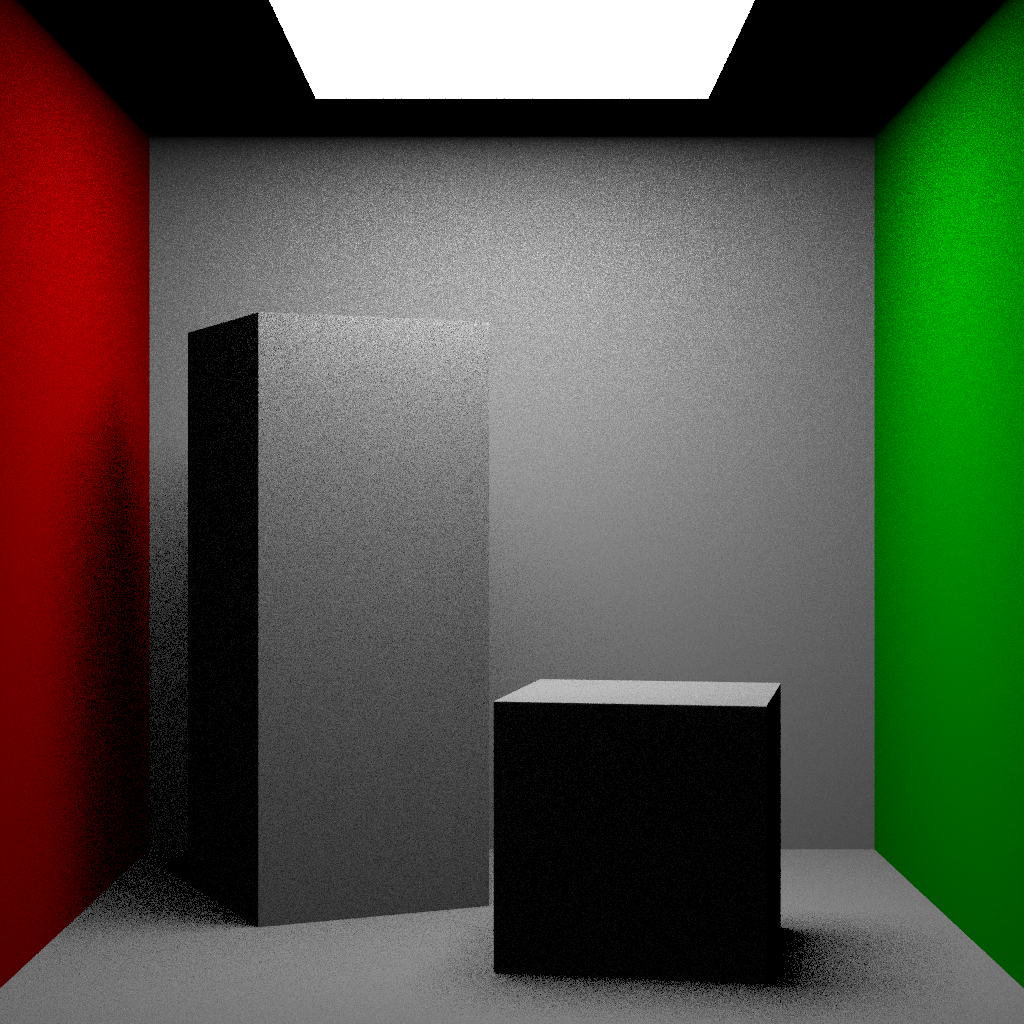
\includegraphics[width=\textwidth]{q3/med_2_10.png}
      \caption{Rendering of Medium Area Light, at 10 SPP}
  \end{minipage}
  \hfill
  \begin{minipage}[t]{.3\textwidth}
      \centering
      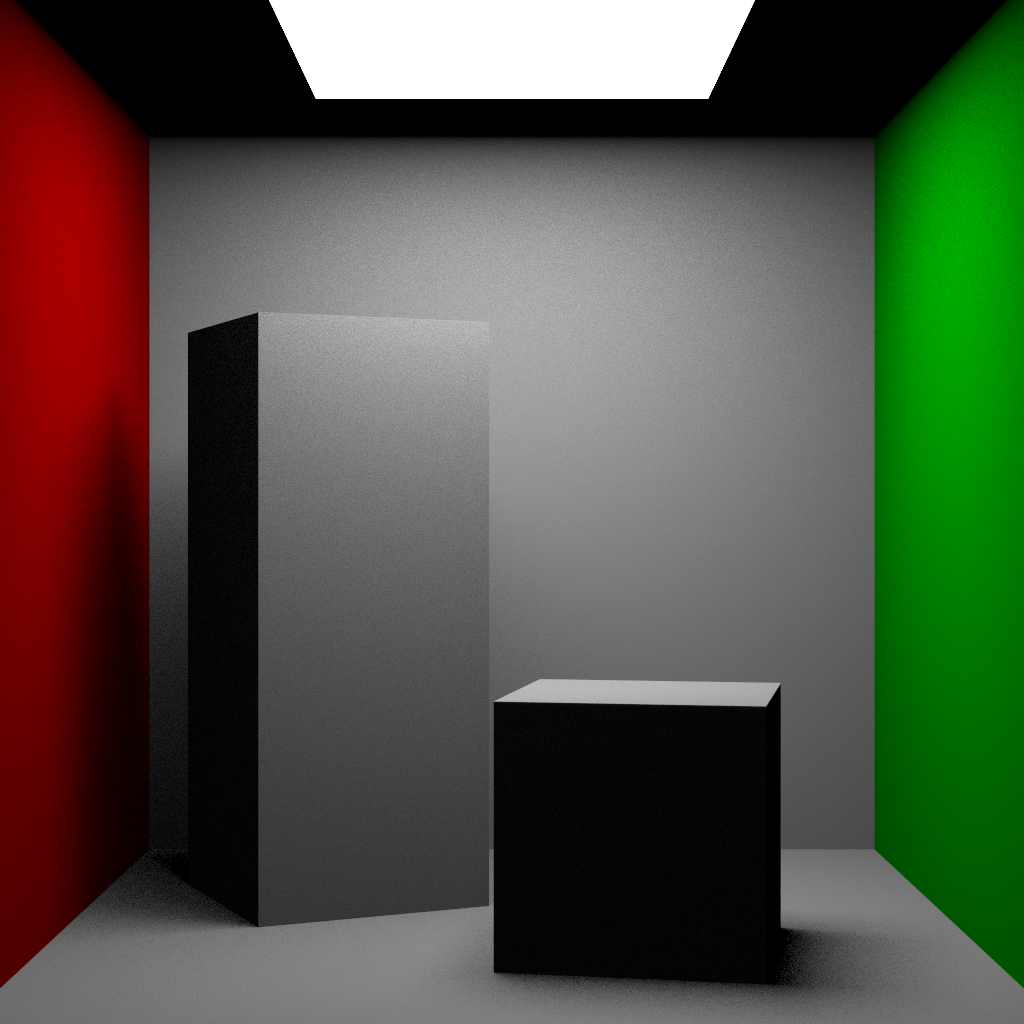
\includegraphics[width=\textwidth]{q3/med_2_100.png}
      \caption{Rendering of Medium Area Light, at 100 SPP}
  \end{minipage}
  \hfill
  \begin{minipage}[t]{.3\textwidth}
      \centering
      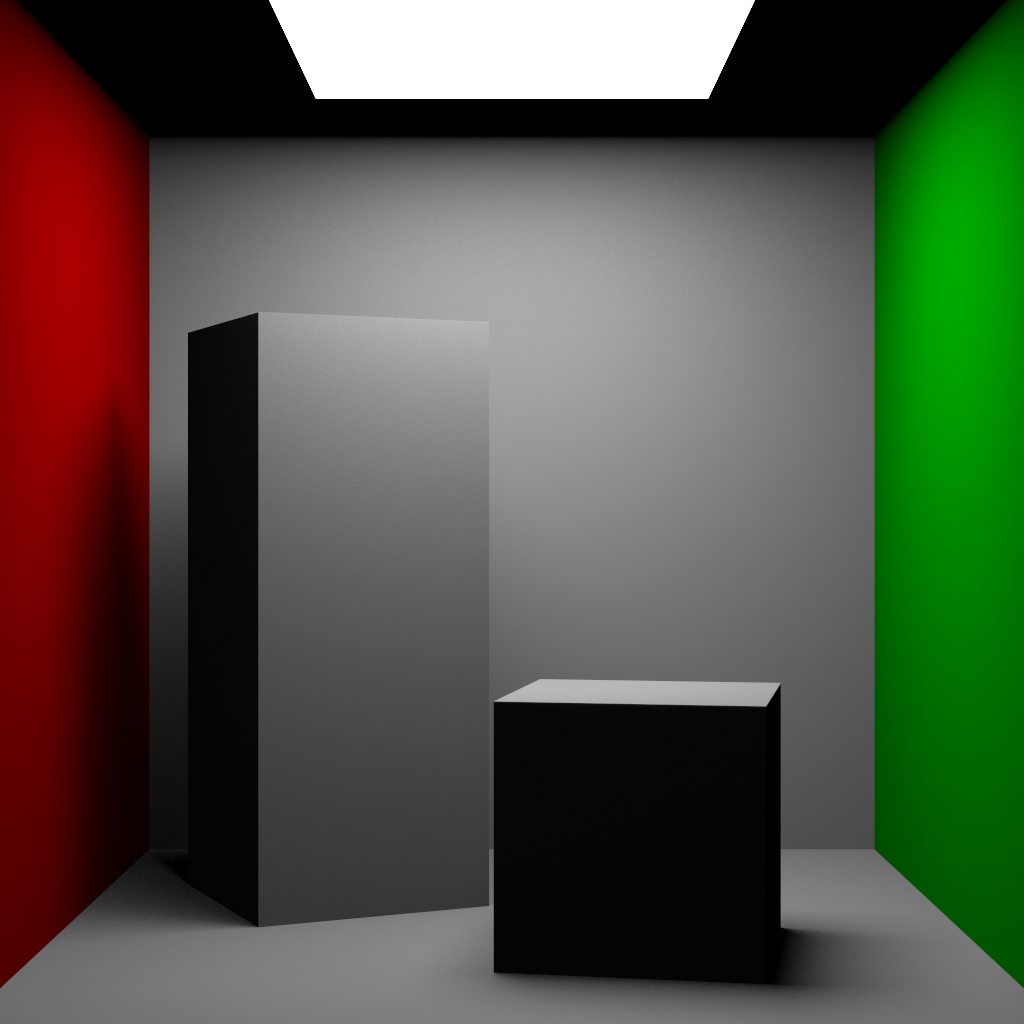
\includegraphics[width=\textwidth]{q3/med_2_1000.png}
      \caption{Rendering of Medium Area Light, at 1000 SPP}
  \end{minipage}
\end{figure}

\begin{figure}[H]
  \begin{minipage}[t]{.3\textwidth}
      \centering
      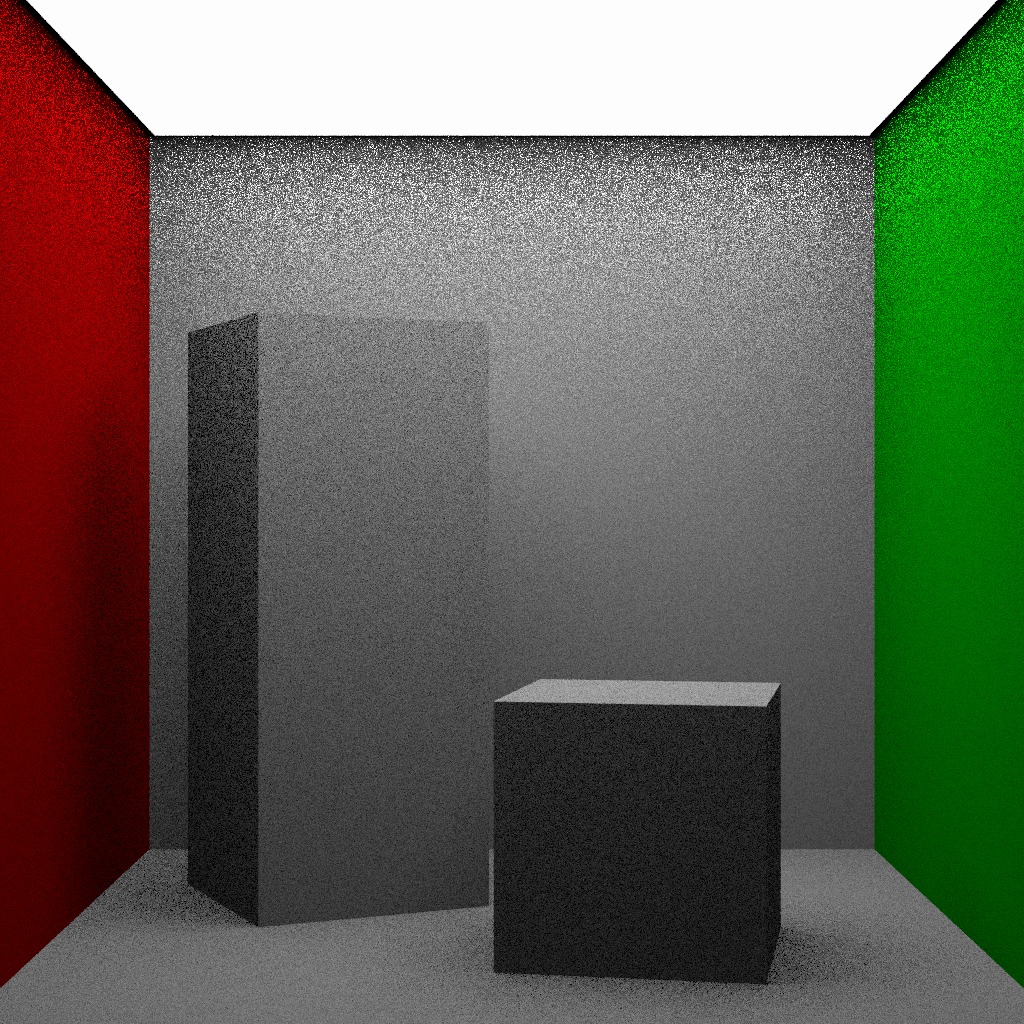
\includegraphics[width=\textwidth]{q3/big_2_10.png}
      \caption{Rendering of Big Area Light, at 10 SPP}
  \end{minipage}
  \hfill
  \begin{minipage}[t]{.3\textwidth}
      \centering
      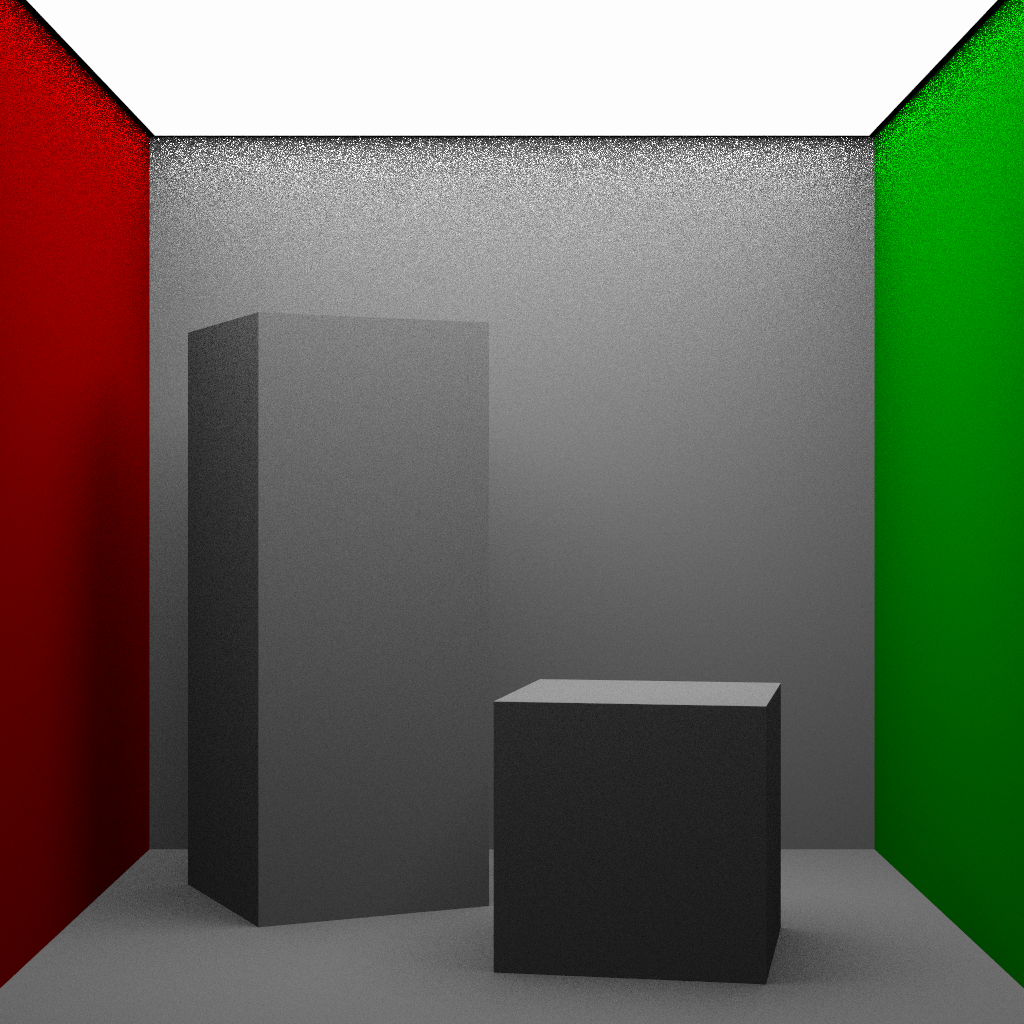
\includegraphics[width=\textwidth]{q3/big_2_100.png}
      \caption{Rendering of Big Area Light, at 100 SPP}
  \end{minipage}
  \hfill
  \begin{minipage}[t]{.3\textwidth}
      \centering
      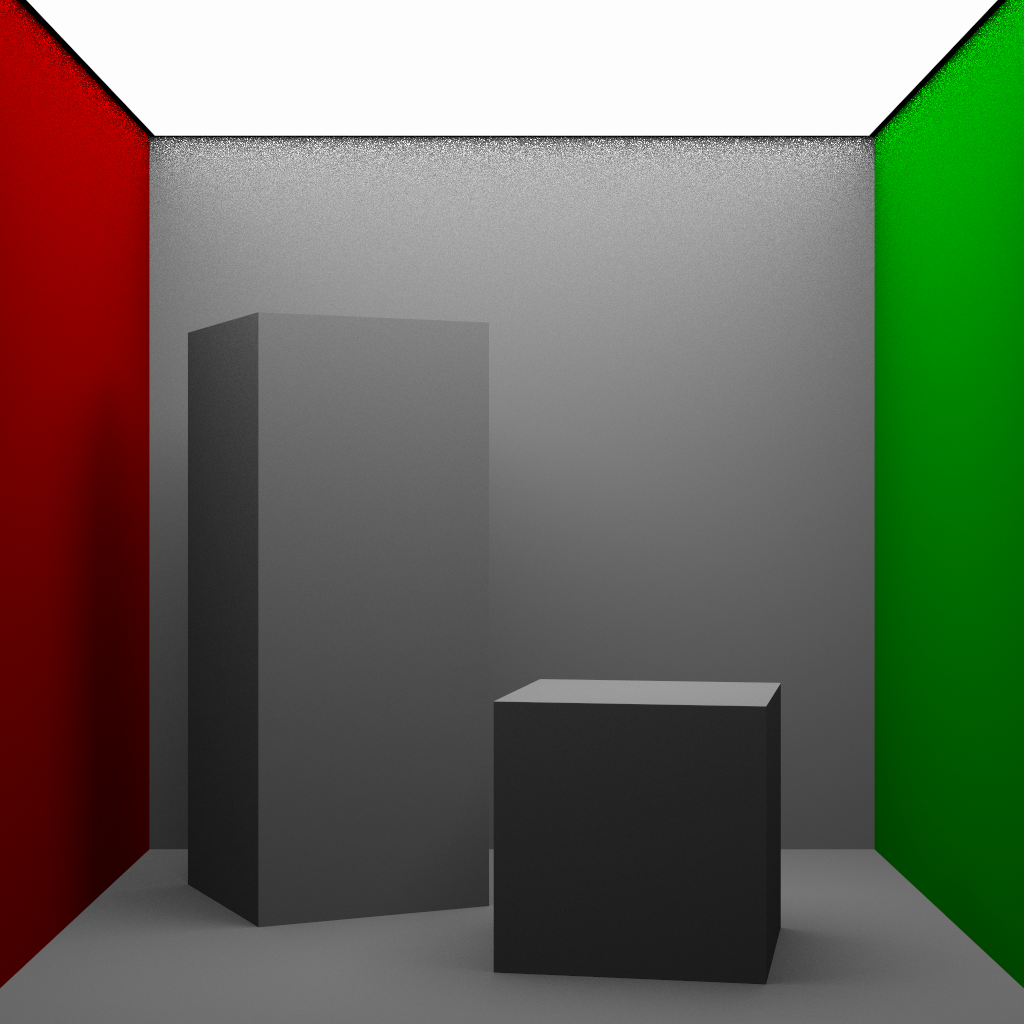
\includegraphics[width=\textwidth]{q3/big_2_1000.png}
      \caption{Rendering of Big Area Light, at 1000 SPP}
  \end{minipage}
\end{figure}

\begin{figure}[H]
  \begin{minipage}[t]{.3\textwidth}
      \centering
      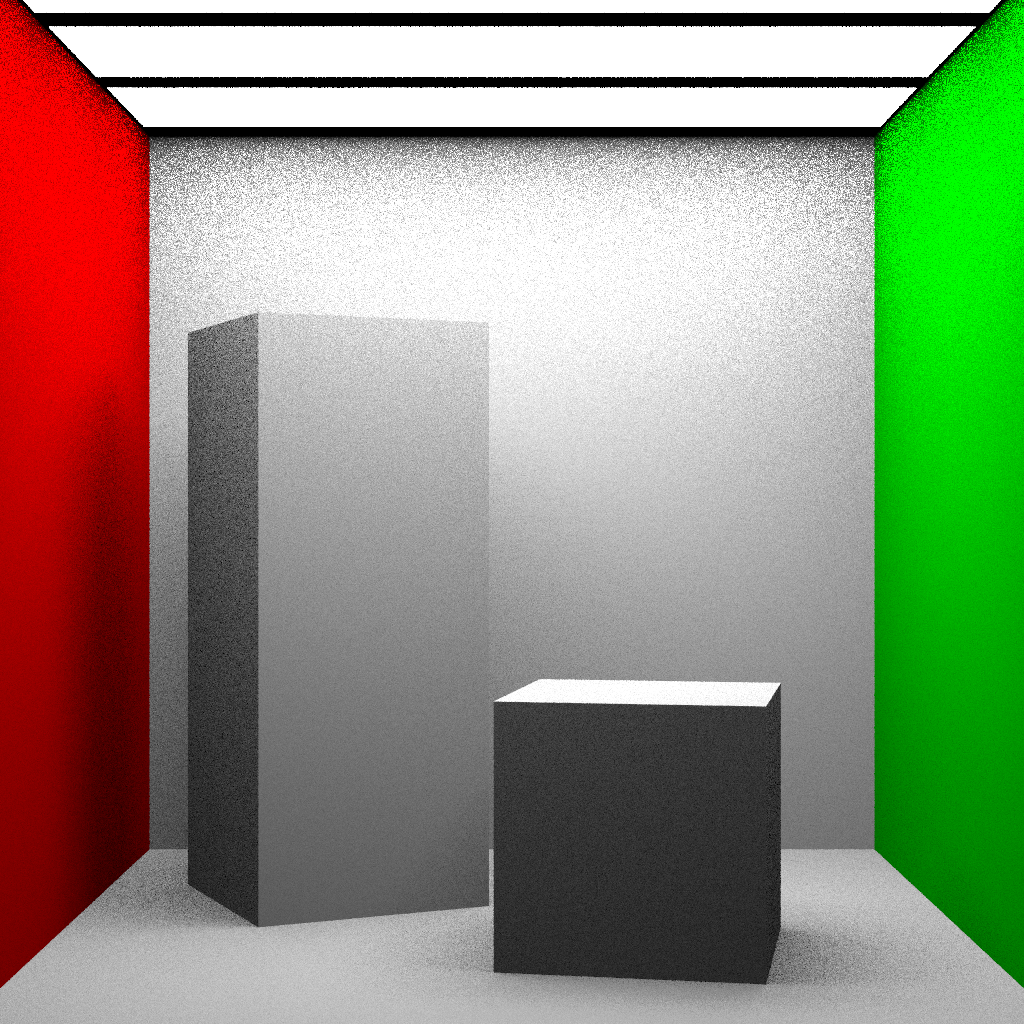
\includegraphics[width=\textwidth]{q3/many_2_10.png}
      \caption{Rendering of Many Area Lights, at 10 SPP}
  \end{minipage}
  \hfill
  \begin{minipage}[t]{.3\textwidth}
      \centering
      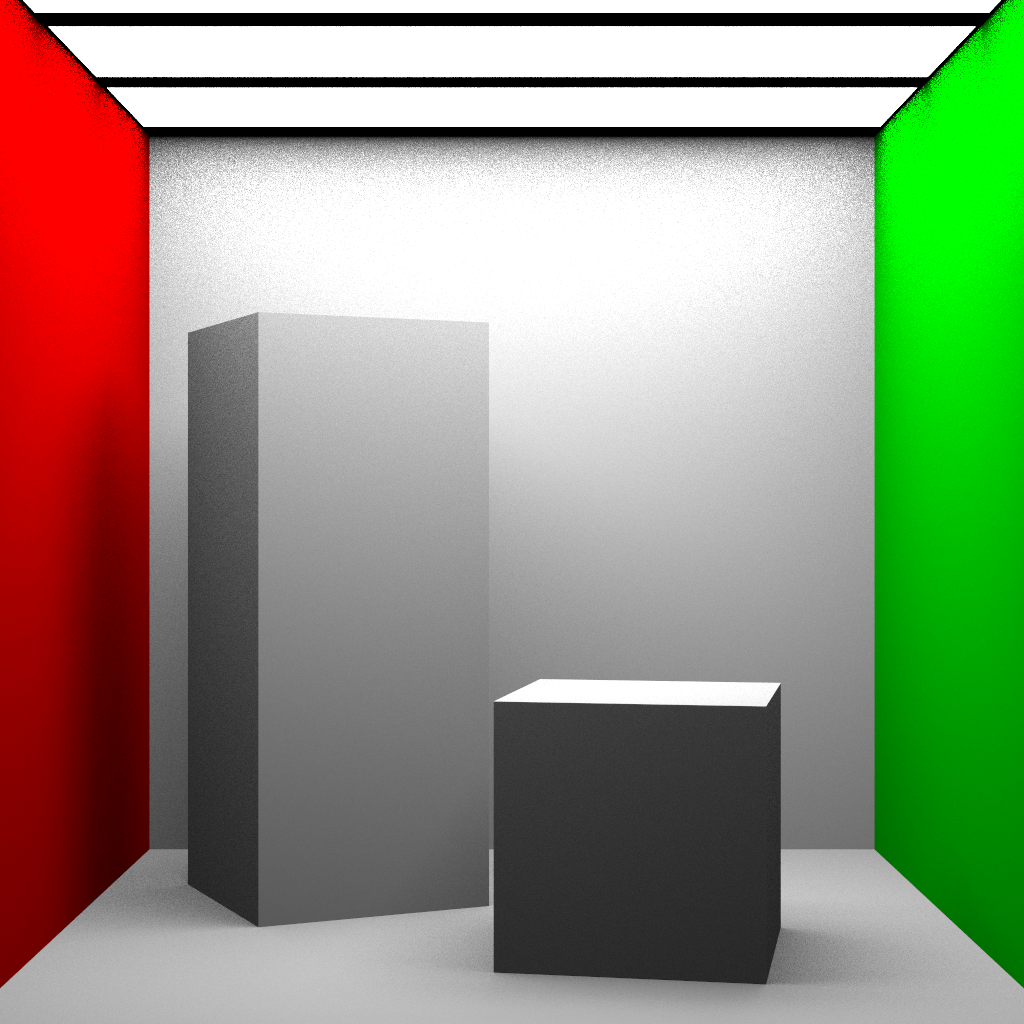
\includegraphics[width=\textwidth]{q3/many_2_100.png}
      \caption{Rendering of Many Area Lights, at 100 SPP}
  \end{minipage}
  \hfill
  \begin{minipage}[t]{.3\textwidth}
      \centering
      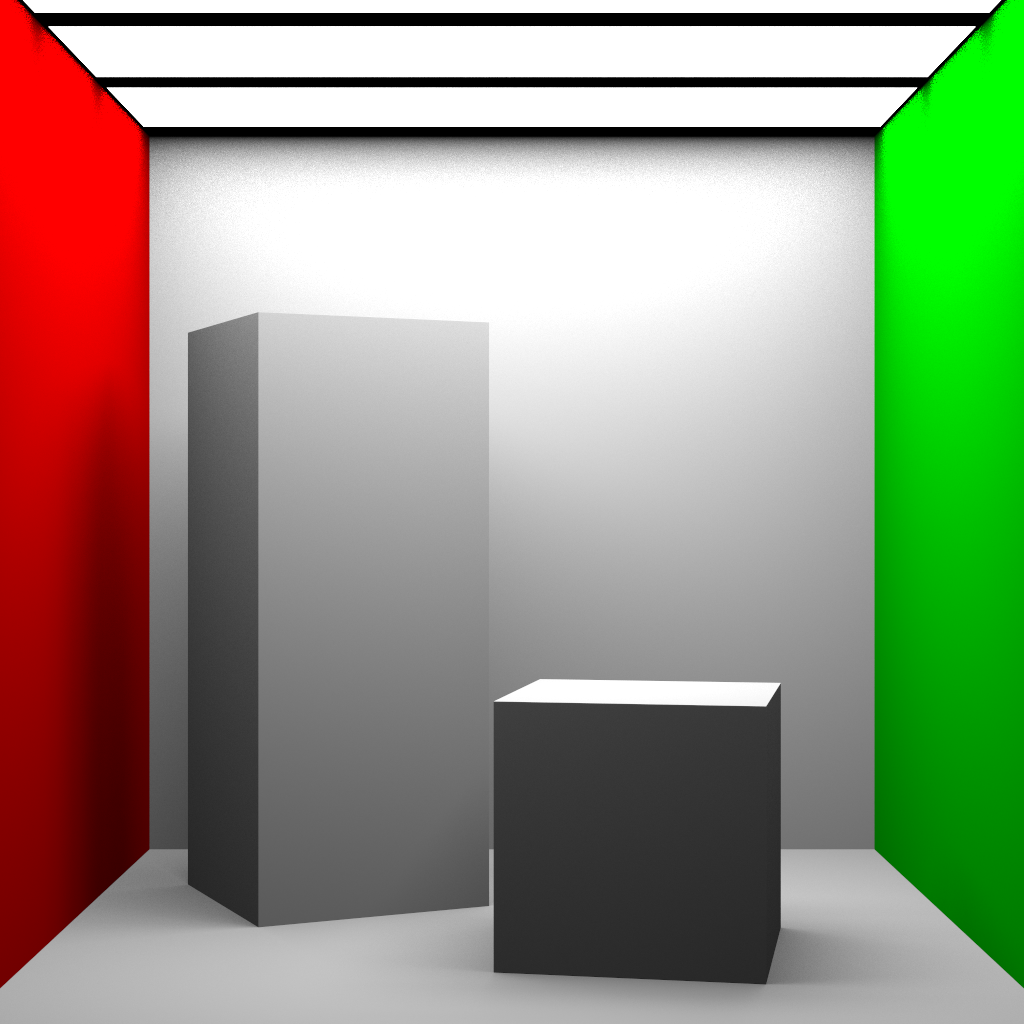
\includegraphics[width=\textwidth]{q3/many_2_1000.png}
      \caption{Rendering of Many Area Lights, at 1000 SPP}
  \end{minipage}
\end{figure}

\section{Follow-Up Questions}

\subsection{Why can't we render point and directional lights with uniform hemisphere sampling or cosine weighted sampling?}

Suppose for the sake of contradiction, we could use uniform hemisphere or cosine weighted sampling, for shading with point and directional lights. This would require us to sample a direction $\omega_i$, such that $V(\textbf{x}, \omega_i) = 1$. We know that for point and directional lights, there can exist only a unique value of $\omega_i$, that satisifies this constraint for any given $\textbf{x}$, in particular $p' - \textbf{x}$, and $-\omega'$ respectively (as per the notation used in slides). The probability of sampling this unique direction from a continuous distribution is zero. Thus, our rendering may never converge to the ground truth, with any arbitrary number of samples.

\subsection{Why does the noise increase for the same number of samples in the case of uniform hemisphere and cosine weighted sampling as the size of the area light decreases?}

The sampling distribution in both the cases depends only on the normal at the intersection point, which defines the upper hemisphere at the intersection. Evidently, it is independent of the size of the concerned area lights. As the size of the area light decreases, the probability of these independently sampled directions $\omega_i$ intersecting the area light, i.e. $V(\textbf{x}, \omega_i) = 1$, decreases. Thus, we require more number of samples to locate the area light for proper shading, and converge to the ground truth. Failure to do so leaves us with the perception of noise in the rendering.

\end{document}
